%\documentclass[lineno]{jfm}
\documentclass[lineno]{JFM-FLM_Au}
\usepackage{subfigure}

%\usepackage{showframe}

\newtheorem{lemma}{Lemma}
\newtheorem{corollary}{Corollary}

\lefttitle{Author 1 et al.}
\righttitle{Journal of Fluid Mechanics}

\title{JFM {\LaTeX} submission template}

\author{Author 1\aff{1}, Author 2\aff{1} \and Author 3\aff{2}}

\affiliation{\aff{1}Department, Institution, City, Country
\aff{2}Department, Institution, City, Country}

\corresau{Author 1, email}

\begin{document}
\maketitle

\begin{abstract}
This file contains information for authors planning to submit a paper to the {\it Journal of Fluid Mechanics}. The document was generated in {\LaTeX} using the JFM class file and supporting files provided on the JFM website \href{https://www.cambridge.org/core/journals/journal-of-fluid-mechanics/information/author-instructions/preparing-your-materials}{here}, and the source files can be used as a template for submissions (please note that this is mandatory for {\it JFM Rapids}). Full author instructions can be found on the \href{https://www.cambridge.org/core/journals/journal-of-fluid-mechanics/information/author-instructions}{JFM website}. The present paragraph appears in the \verb}abstract} environment. All papers should feature a single-paragraph abstract of no more than 250 words which must not spill onto the second page of the manuscript.
\end{abstract}

\begin{keywords}
Authors should not enter keywords on the manuscript, as these must be chosen by the author during the online submission process and will then be added during the typesetting process (see \href{https://www.cambridge.org/core/services/aop-file-manager/file/61436b61ff7f3cfab749ce3a/JFM-Keywords-Sept-2021.pdf.}{Keyword PDF} for the full list).  Other classifications will be added at the same time.
\end{keywords}

%{\bf MSC Codes }  {\it(Optional)} Please enter your MSC Codes here

\section{Rigid case}
\begin{figure}[htb]
	\begin{center}
		% specify width as 80% of the width of the text on the page
		% we can also specify a width in centimetres, e.g. [width=8cm]
		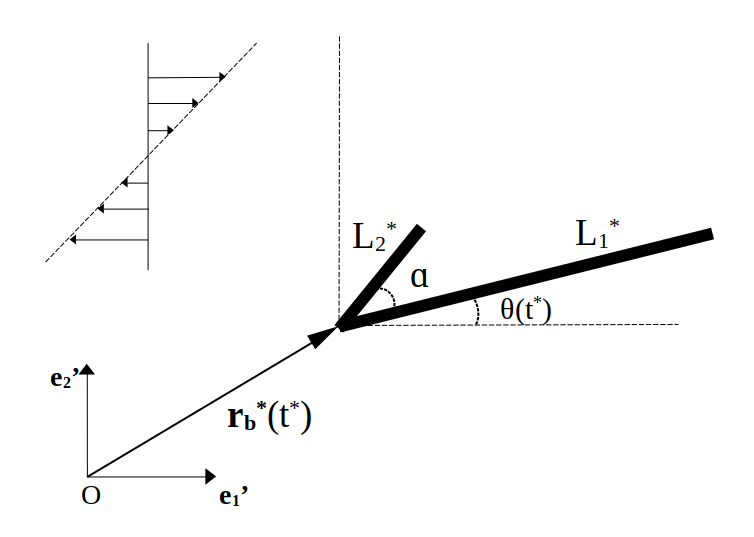
\includegraphics[width=0.5\textwidth]{plot/rigid_case/schematic_rigid_configuration.png}
		\caption{Schematics of the geometry of boomerang-shaped rigid fibres.}
		\label{fig:21}
	\end{center}
	%	\setlength{\abovecaptionskip}{-0.5 cm}
\end{figure}

\begin{figure}[htbp]
	\centering
	\begin{minipage}[t]{0.4\textwidth}
		\centering
		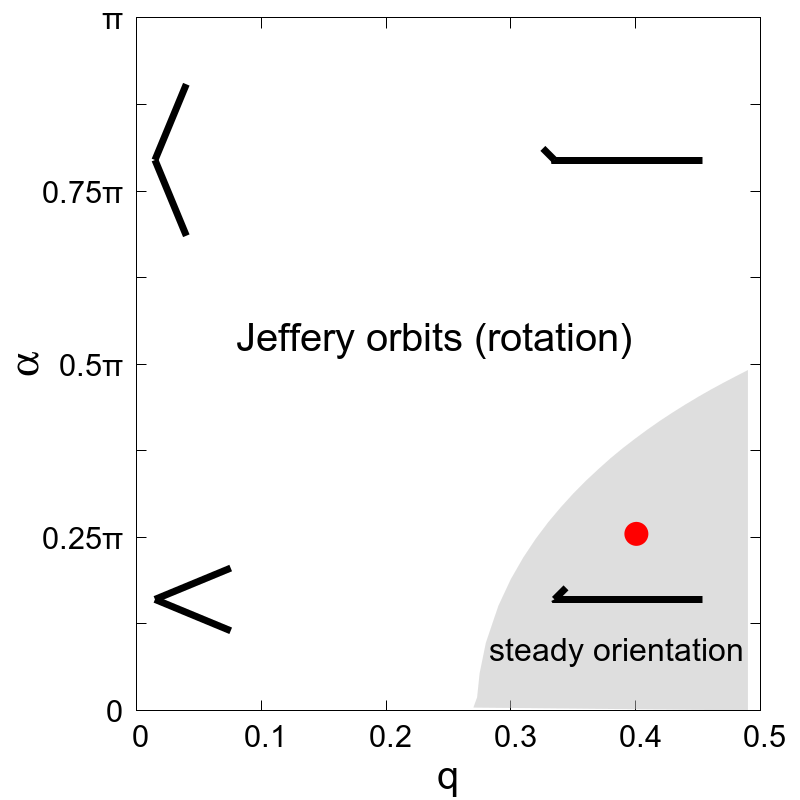
\includegraphics[width=\linewidth]{plot/rigid_case/q_alpha_plot_with_point.png}
	\end{minipage}
	\hfill
	\begin{minipage}[t]{0.58\textwidth}
		\centering
		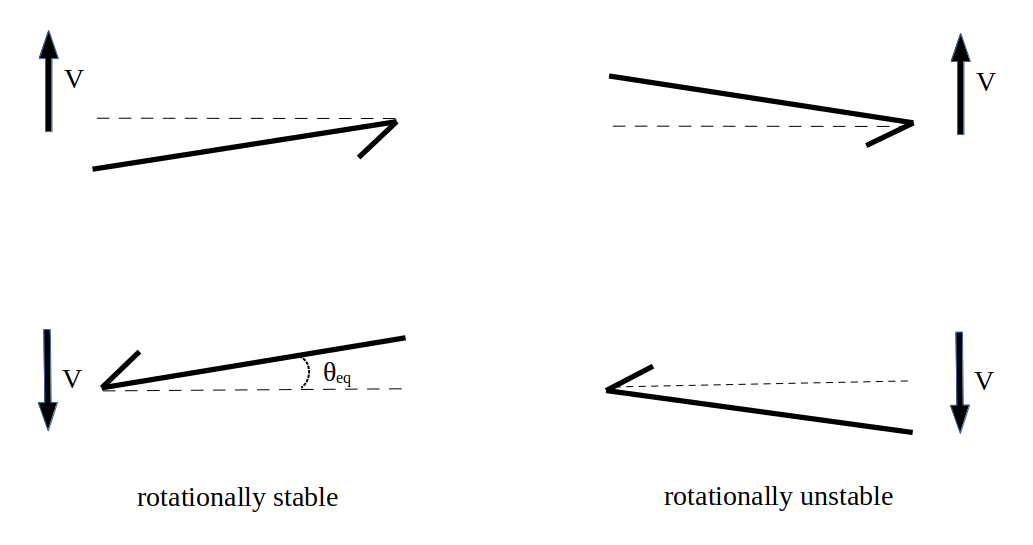
\includegraphics[width=\linewidth]{plot/rigid_case/q_alpha_plot_with_point_four_equilibria.png}
	\end{minipage}
	\caption{Left: Two regions in $q-\alpha$ parameter space indicate distinct types of motion for rigid fibres. Right: The case corresponding to the red point in the left plot. In the grey region, there exist four equilibria in total—two stable and two unstable. The two stable equilibria differ by an angle of $\pi$, drifting at the same speed but in opposite directions; the same applies to the two unstable ones.}
	\label{fig:18}
\end{figure}


\section{Theoretical Framework}

\subsection{Fluid-solid interaction}
Generally speaking, we will investigate a two-dimensional problem concerning the deformation and motion of a slender elastic fibre in shear flow at a low Reynolds number, focussing on the fibre's orientation and trajectory in the fluid. As this project concerns both fluid and solid mechanics, we will introduce these two components separately and then couple them to discuss the fluid-solid interaction.
\subsubsection{Fluid mechanics}
We set the undeformed slender elastic fibre clamped at the origin of the laboratory reference frame $\{\mathbf{e'_1}, \mathbf{e'_2}, \mathbf{e'_3}\}$ as
$\mathbf{r}_0^*(\xi^*)=(0,\xi^*)^T$, where $\xi^*\in [0,\mathcal{L}]$. We then assume that its deformed state is given by $\mathbf{R}_0^*(\xi^*,t^*)$. 
Final position of the deformed fibre after translation and rotation is determined as follows:
\begin{equation}
	\label{eqn:19}
	\mathbf{R}^*(\xi^*,t^*)=\mathbf{\mathcal{R}}\,\mathbf{R}_0^*(\xi^*,t^*)+\mathbf{r}_b^*(t^*),
\end{equation}
where $\mathbf{\mathcal{R}}=\left(\begin{aligned}
	&\cos(\phi(t^*))\quad -\sin(\phi(t^*)) \\
	&\sin(\phi(t^*))\quad \cos(\phi(t^*))
\end{aligned}\right)$ is the rotation matrix with $\phi(t^*)$ which measures the fibre's inclination as shown in Figure \ref{fig:5}, and $\mathbf{r}_b^*(t^*)=\left(\begin{aligned}
	&X(t^*) \\
	&Y(t^*)
\end{aligned}\right)$ represents the translation of the fibre. Note that inclination $\phi(t^*)$ refers to the actual rotational angle of the object. From Figure \ref{fig:5}, we can easily derive the relationship between orientation and inclination as follows:
\begin{equation}
	\label{eqn:20}
	\theta(t^*)=\frac{\pi}{2}-\phi(t^*).
\end{equation}
\begin{figure}[htb]
	\begin{center}
		% specify width as 80% of the width of the text on the page
		% we can also specify a width in centimetres, e.g. [width=8cm]
		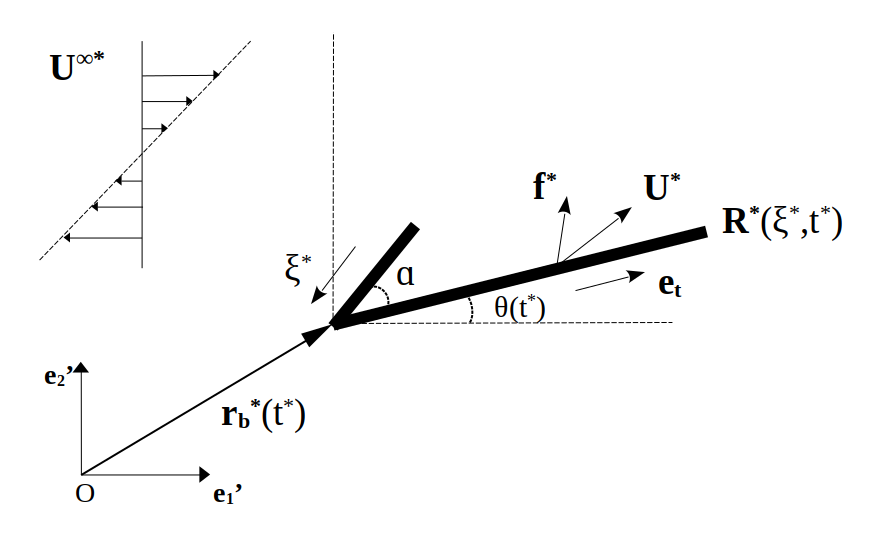
\includegraphics[width=0.5\textwidth]{plot/rigid_case/schematic_rigid_configuration_color0_old.png}
		\caption{Schematics of the geometry of boomerang-shaped rigid fibres.}
		\label{fig:23}
	\end{center}
	%	\setlength{\abovecaptionskip}{-0.5 cm}
\end{figure}
\begin{figure}[htb]
	\begin{center}
		% specify width as 80% of the width of the text on the page
		% we can also specify a width in centimetres, e.g. [width=8cm]
		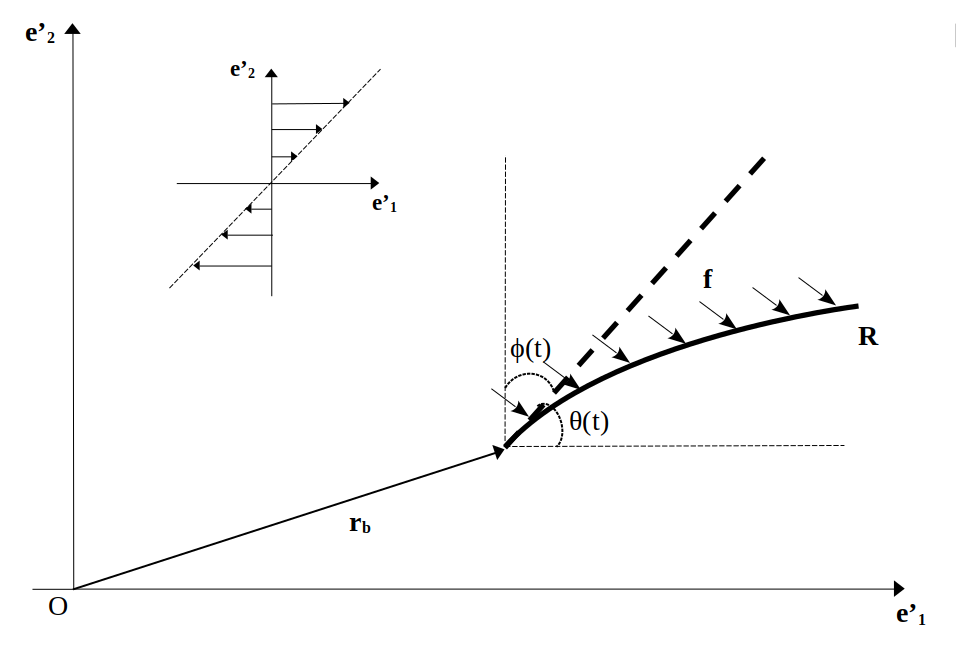
\includegraphics[width=0.8\textwidth]{plot/fluid_general.png}
		\caption{Schematic of a slender elastic fibre in the deformed state in shear flow. The dashed black line represents its undeformed configuration.}
		\label{fig:5}
	\end{center}
	%	\setlength{\abovecaptionskip}{-0.5 cm}
\end{figure}
Since we consider a slender elastic fibre immersed in shear flow, the velocity of the background flow is given by
\begin{equation}
	\label{eqn:21}
	\mathbf{U}^{\infty*}(\mathbf{R}^*(\xi^*,t^*))=\dot{\gamma}\left(\mathbf{R}^*(\xi^*,t^*)\cdot\mathbf{e}_y\right)\cdot\mathbf{e}_x,
\end{equation}
where $\mathbf{e}_x=(1,0)^T$ and $\mathbf{e}_y=(0,1)^T$ are both unit vectors. Then, the fibre's velocity from kinematics is 
\begin{equation}
	\label{eqn:22}
	\mathbf{U}^*=\frac{\partial\mathbf{R}^*(\xi^*,t^*)}{\partial t^*}.
\end{equation}
Let us define a tangential vector to surface of the fibre:
\begin{equation}
	\label{eqn:23}
	\mathbf{e}_t=\frac{1}{|\frac{\partial\mathbf{R}^*(\xi^*,t^*)}{\partial\xi^*}|}\frac{\partial\mathbf{R}^*(\xi^*,t^*)}{\partial\xi^*}.
\end{equation}
From the slender body theory, the traction is obtained as flows:
\begin{equation}
	\label{eqn:24}
	\mathbf{f}^*=c_\perp\left(\mathbf{I}-\frac{1}{2}\mathbf{e}_t\mathbf{e}_t\right)\cdot(\mathbf{U}^{\infty*}-\mathbf{U}^*),
\end{equation}
where $c_\perp=\frac{4\pi\mu}{\ln{\frac{1}{\epsilon}}}$ is the drag coefficient. 

We non-dimensionalise the variables mentioned in this section using the following basic relationships (we set the total length
of the fibre as the characteristic length $\mathcal{L}$ and define the time scale as $\frac{1}{\dot{\gamma}}$ , where $\dot{\gamma}$ is the shear rate.) :
\begin{equation}
	\label{eqn:25}
	\xi^*=\mathcal{L}\xi, \quad t^*=\frac{1}{\dot{\gamma}}\,t.
\end{equation}
Note that the non-dimensional variables are identified without asterisks.
Hence, the relationship between dimensional and non-dimensional variables are given by
\begin{equation}
	\label{eqn:26}
	(\mathbf{r}_0^*, \mathbf{r}_b^*, \mathbf{R}_0^*, \mathbf{R}^*)^T=\mathcal{L}\cdot(\mathbf{r}_0, \mathbf{r}_b, \mathbf{R}_0, \mathbf{R})^T,
\end{equation}
\begin{equation}
	\label{eqn:27}
	\mathbf{U}^{\infty*}=\mathcal{L}\dot{\gamma}\mathbf{U}^{\infty}, \quad \mathbf{U}^*=\mathcal{L}\dot{\gamma}\mathbf{U},
\end{equation}
\begin{equation}
	\label{eqn:28}
	\mathbf{f}^*=c_\perp\,\mathcal{L}\,\dot{\gamma}\,\left(\mathbf{I}-\frac{1}{2}\mathbf{e}_t\mathbf{e}_t\right)\cdot(\mathbf{U}^{\infty}-\mathbf{U})=c_\perp\,\mathcal{L}\,\dot{\gamma}\,\mathbf{f}_{f},
\end{equation}
where 
\begin{equation}
	\label{eqn:101}
	\begin{aligned}
		\mathbf{f}_f=&\left(\mathbf{I}-\frac{1}{2}\mathbf{e}_t\mathbf{e}_t\right)\cdot(\mathbf{U}^{\infty}(t)-\mathbf{U}(t))\\
		=&\left(\mathbf{I}-\frac{1}{2}\mathbf{e}_t\mathbf{e}_t\right)\cdot\Big((\mathbf{\mathbf{R}}(\xi,t)\cdot\mathbf{e}_y)\cdot\mathbf{e}_x-\frac{\partial\mathbf{R}(\xi,t)}{\partial t}\Big)
	\end{aligned}
\end{equation}
is the non-dimensional fluid traction. 

\subsubsection{Solid mechanics}
We are considering the fluid-solid interaction, so next we will focus on the part related to solid mechanics. This report employs geometrically nonlinear Kirchhoff-Love beam theory with incrementally linear constitutive equations to describe the deformation issues of elastic beams subjected to forces in fluid. We define the deformation of the beam as the dimensionless centreline displacement, $\mathbf{\omega} = \frac{\mathbf{\omega}^*}{\mathcal{L}}$. The position of a material point on the beam's centerline is denoted by 
\begin{equation}
	\label{eqn:61}
	\mathbf{r}_0(\xi^1, \xi^2=0)=\mathbf{r}^0_0(\xi^1),\quad \xi^1\in [0,1].
\end{equation}
Then the position of an arbitrary point in the undeformed beam is given by 
\begin{equation}
	\label{eqn:62}
	\mathbf{r}_0(\xi^1, \xi^2)=\mathbf{r}^0_0(\xi^1)+\xi^2\mathbf{n},\quad \xi^2\in [-\frac{h}{2},\frac{h}{2}],
\end{equation}
where $\mathbf{n}=(1,0)^T$ is the normal vector to the undeformed centerline, and $\frac{h}{2}=\frac{h^*}{2\mathcal{L}}$ is the non-dimensional radius of the cross section of the beam. After the deformation, the previous position $\mathbf{r}^0_0(\xi^1)$ in the undeformed reference configuration is transformed to a new position 
\begin{equation}
	\label{eqn:63}
	\mathbf{R}^0_0(\xi^1)=\mathbf{r}^0_0(\xi^1)+\mathbf{\omega}(\xi^1).
\end{equation}
We decompose the displacement $\mathbf{\omega}$ into the undeformed basis:
\begin{equation}
	\label{eqn:64}
	\mathbf{\omega}=\omega^1\mathbf{a}_1+\omega^2\mathbf{a}_2,
\end{equation}
where $\mathbf{a}_1=\frac{\partial \mathbf{r}^0_0}{\partial\xi^1}$ and $\mathbf{a}_3=\mathbf{n}$. The Kirchhoff-Love assumption states that material lines, which were normal to the undeformed centreline, remain normal to the deformed centreline and remain unstretched. Therefore, an arbitrary material point $\mathbf{r}_0$ after deformation is given by 
\begin{equation}
	\label{eqn:65}
	\mathbf{R}_0(\xi^1,\xi^2)=\mathbf{R}^0_0(\xi^1)+\xi^2\mathbf{N},
\end{equation}
where $\mathbf{N}$ is the normal to the deformed configuration.

We then give the non-dimensional equation by scaling the stresses and the applied traction on the beam's bending stiffness:
\begin{equation}
	\label{eqn:30}
	\left(\begin{aligned}
		&\mathbf{f^*} \\
		&\mathbf{\sigma}_0^*
	\end{aligned}\right)
	=\frac{K}{\mathcal{L}^3}\left(\begin{aligned}
		&\mathbf{f}_{s} \\
		&\mathbf{\sigma}_0
	\end{aligned}\right),
\end{equation}
where $\mathbf{f}_{s}$ is the non-dimensional solid traction and $\sigma^*_0$ indicates the prestress of the elastic beam.
The non-dimensional form of the principle of virtual displacements that governs the beams deformation is then given by
\begin{equation}
	\label{eqn:31}
	\int^1_0 \left[(\sigma_0+\gamma)\delta\gamma+\frac{1}{12}h^2\kappa\delta\kappa-\frac{1}{h}\sqrt{\frac{A}{a}}\,\mathbf{f}_{s}\cdot \delta \mathbf{R}_0
	\right]\,\sqrt{a}\,d\xi=0,
\end{equation}
where 
\begin{equation}
	\label{eqn:32} a=\frac{\partial\mathbf{r}_0}{\partial\xi}\cdot\frac{\partial\mathbf{r}_0}{\partial\xi}, A=\frac{\partial\mathbf{R}_0}{\partial\xi}\cdot\frac{\partial\mathbf{R}_0}{\partial\xi}
\end{equation}
denote the squares of the lengths of infinitesimal material line elements in the undeformed and deformed configurations, respectively.
Also, considering undeformed and deformed ones, we have 
\begin{equation}
	\label{eqn:33}
	ds=\sqrt{a}\,d\xi,\,dS=\sqrt{A}\,d\xi.
\end{equation}
$A$ and $a$ could be understood as the "$1\times1$ metric tensors" of the beam's centerline, representing the deformed and undeformed configurations, respectively. 
The ratio $\sqrt{\frac{A}{a}}$ signifies the "extension ratio" or "stretch" of the beam's centerline. We define the curvature of the beam's centerline prior to and following deformation as represented by 
\begin{equation}
	\label{eqn:34}
	b=\mathbf{n}\cdot\frac{d^2\mathbf{r}_0}{d\xi^2},\,B=\mathbf{N}\cdot\frac{\partial^2\mathbf{R}_0}{\partial\xi^2}.
\end{equation}
The "$1\times1$" strain and bending "tensors" $\gamma$ and $\kappa$ are obtained by
\begin{equation}
	\label{eqn:35}
	\gamma=\frac{1}{2}(A-a),\,\kappa=-(B-b).
\end{equation}

Since the elastic beam is initially clamped at the origin, the boundary conditions are
\begin{equation}
	\label{eqn:58}
	\begin{aligned}
		&\mathbf{R}_0(\xi=0)\cdot\mathbf{e}_x=0,\\
		&\mathbf{R}_0(\xi=0)\cdot\mathbf{e}_y=0,\\
		&\frac{d\left(\mathbf{R}_0(\xi=0)\cdot\mathbf{e}_x\right)}{d\xi}=0.
	\end{aligned}
\end{equation}

\subsubsection{Fluid–solid coupling}
The no-slip boundary condition requires that the velocity of the fluid on the surface of the beam matches the velocity of the beam at that location. Hence, the boundary condition is 
\begin{equation}
	\label{eqn:100}
	\mathbf{u}=\frac{\partial \mathbf{R}(\xi,t)}{\partial t}.
\end{equation}

Recall that in $\eqref{eqn:28}$, we use slender body theory to evaluate the traction exerted by the fluid on the beam as
\begin{equation}
	\label{eqn:102}
	\mathbf{f}^*=c_\perp\,\mathcal{L}\,\dot{\gamma}\,\mathbf{f}_{f}.
\end{equation}
From \eqref{eqn:30}, the applied traction on beam is 
\begin{equation}
	\label{eqn:103}
	\mathbf{f}^*=\frac{K}{\mathcal{L}^3}\,\mathbf{f}_{s}.
\end{equation}
Hence, the fluid applies traction to the beam, and the loading term in the solid equation \eqref{eqn:31} are expressed by
\begin{equation}
	\label{eqn:37}
	\mathbf{f}_{s}=\frac{c_\perp\,\mathcal{L}^4\,\dot{\gamma}}{K}\,\mathbf{f}_{f}.
\end{equation}
Then, we define the coefficient in \eqref{eqn:37} as $\mathcal{I}$, which represents the fluid-solid interaction parameter (FSI parameter) and is expressed as:
\begin{equation}
	\label{eqn:38}
	\mathcal{I}=\frac{c_\perp\,\mathcal{L}^4\,\dot{\gamma}}{K}.
\end{equation}
It quantifies the degree or strength of the interaction between the fluid and the solid within the system.


\subsection{Governing equations}
Initially, the elastic beam is clamped at the origin, denoted by $\mathbf{r}_0(\xi)=(0,\xi)^T,\,\xi\in [0,1]$. Next, a traction $\mathbf{f}_s=\mathcal{I}\,\mathbf{f}_0$  is applied to it, causing deformation denoted as $\mathbf{R}_0(\xi,t)$. Substituting 
$\mathbf{r}_0(\xi), \mathbf{f}_s$ and $\mathbf{R}_0(\xi,t)$ into the beam's governing equation $\eqref{eqn:31}$, we obtain the following equation:
\begin{equation}
	\label{eqn:48}
	\mathbf{\mathcal{S}}\Big(\mathbf{R}_0(\xi,t);\mathbf{f}_0,\mathbf{r}_0(\xi)\Big)=0,
\end{equation}
where $\mathbf{R}_0(\xi,t)$ is the unknown and $\mathbf{\mathcal{S}}(\cdot)$ indicates the left hand side of $\eqref{eqn:31}$.
Subsequently, according to $\eqref{eqn:19}$, a translation and rotation are applied to 
$\mathbf{R}_0(\xi,t)$, yielding $\mathbf{R}(\xi,t)$ as:
\begin{equation}
	\label{eqn:49}
	\mathbf{R}(\xi,t)=\mathbf{\mathcal{R}}(t)\,\mathbf{R}_0(\xi,t)+\mathbf{r}_b(t).
\end{equation}
We compute the fluid traction $\mathbf{f}_f$ acting on the beam $\mathbf{R}(\xi,t)$ based on $\eqref{eqn:101}$. Then, we rotate this fluid traction $\mathbf{f}_f$ back by angle $\phi(t)$ while keeping its magnitude unchanged, obtaining traction $\mathbf{f}_0$. Hence, the relationship between $\mathbf{f}_0$ and $\mathbf{f}_f$ is 
\begin{equation}
	\label{eqn:50}
	\mathbf{f}_0=\mathbf{\mathcal{R}}^{-1}\,\mathbf{f}_f,
\end{equation}
where $\mathbf{\mathcal{R}}^{-1}$ is the inverse of the rotation matrix. Then, the solid traction, which serves as the loading term in the beam equation, is represented as 
\begin{equation}
	\label{eqn:67}
	\mathbf{f}_s=\mathcal{I}\,\mathbf{f}_0=\mathcal{I}\,\left(\mathbf{\mathcal{R}}^{-1}\,\mathbf{f}_f\right).
\end{equation}
From $\eqref{eqn:19}$ and $\eqref{eqn:101}$, we know that the traction $\textbf{f}_f$ is the function of $\textbf{R}_0(\xi,t), X(t), Y(t)$ and $\phi(t)$. Thus, traction $\textbf{f}_0$ is also the function of these variables, that is, $\textbf{f}_0\left(\textbf{R}_0(\xi,t), X(t), Y(t),\phi(t)\right)$. It means that $\eqref{eqn:48}$ can be updated by
\begin{equation}
	\label{eqn:51}
	\mathbf{\mathcal{S}}\Big(\mathbf{R}_0(\xi,t), X(t), Y(t),\phi(t);\mathbf{r}_0(\xi)\Big)=0.
\end{equation}
Note that $\mathbf{r}_0(\xi)=(0,\xi)^T,\,\xi\in [0,1]$ is not the unknown in this equation.

The net drag and net torque acting on the beam $\mathbf{R}(\xi,t)$ in non-dimensional form are 
\begin{equation}
	\label{eqn:52}
	\mathbf{F}=\int^1_0 \mathbf{f}\, \left|\frac{\partial\mathbf{R}}{\partial\xi}\right|\,d\xi, 
\end{equation}
\begin{equation}
	\label{eqn:53}
	\mathbf{T}\cdot\mathbf{e}_z=\left\{\int^1_0 \left[(\mathbf{R}-\mathbf{R}_c)\times \mathbf{f}\,\right]\,\left|\frac{\partial\mathbf{R}}{\partial\xi}\right|\,d\xi\right\}\cdot\mathbf{e}_z,
\end{equation}
where 
\begin{equation}
	\label{eqn:54}
	\mathbf{R}_c=\int^1_0 \mathbf{R}\,\left|\frac{\partial\mathbf{R}}{\partial\xi}\right|\,d\xi
\end{equation}
represents the position of centre of mass. Under the Stokes flow regime, both the fluid and the immersed fibre are assumed to have negligible inertia. As a result, there is no temporal accumulation of momentum, and the system must satisfy the equilibrium conditions at every time instant. We assume that there is no external body force, thus the system must satisfy the conditions of drag-free and torque-free. Hence, we have 
\begin{equation}
	\label{eqn:55}
	\mathbf{F}\,\Big(\mathbf{R}_0(\xi,t), X(t), Y(t), \phi(t)\Big)=\mathbf{0},
\end{equation}
\begin{equation}
	\label{eqn:56}
	\{\mathbf{T}\cdot\mathbf{e}_z\}\,\Big(\mathbf{R}_0(\xi,t), X(t), Y(t), \phi(t)\Big)=0.
\end{equation} 
Combining $\eqref{eqn:51}, \eqref{eqn:55}$ and $\eqref{eqn:56}$, we collect the following equations for unkonwns:
\begin{equation}
	\label{eqn:57}
	\left\{\begin{aligned}
		&\mathbf{\mathcal{S}}\Big(\mathbf{R}_0(\xi,t), X(t), Y(t),\phi(t);\mathbf{r}_0(\xi)\Big)=0\\
		&\mathbf{F}\,\Big(\mathbf{R}_0(\xi,t), X(t), Y(t),\phi(t)\Big)=\mathbf{0}\\
		&\{\mathbf{T}\cdot\mathbf{e}_z\}\,\Big(\mathbf{R}_0(\xi,t), X(t), Y(t),\phi(t)\Big)=0
	\end{aligned}\right.\Longrightarrow \Big(\mathbf{R}_0(\xi,t), X(t), Y(t),\phi(t)\Big).
\end{equation}

\subsection{Equilibrium governing equations}

We are particularly interested in the equilibrium solutions of an elastic fibre in shear flow, rather than the trivial tumbling state. 

\subsubsection{Solutions with constant orientations}
From the rigid fibre case, we assume that an elastic fibre will also undergo a fixed orientation with a uniform drift. Hence, it is worth studying further the solutions with constant orientations (Namely, from \eqref{eqn:20}, we seek the steady solution for inclination $\phi(t)$, $\dot{\phi}(t)=0$), hence the following conditions are made:
\begin{equation}
	\label{eqn:39}
	\overline{\phi}(t)=\phi_{eq},\, \overline{\mathbf{R}_0}(\xi,t)=\mathbf{R}_0(\xi).
\end{equation}
Note that variables with an overbar denote their base state. Thus, from \eqref{eqn:19} we obtain the following expressions in non-dimensional form with the conditions above:
\begin{equation}
	\label{eqn:40}
	\overline{\mathbf{R}}(\xi,t)=\overline{\mathbf{\mathcal{R}}}\,\mathbf{R}_0(\xi)+\overline{\mathbf{r}_b}(t),
\end{equation}
where $\overline{\mathbf{\mathcal{R}}}=\left(\begin{aligned}
	&\cos(\phi_{eq})\quad -\sin((\phi_{eq}) \\
	&\sin((\phi_{eq})\quad \cos((\phi_{eq})
\end{aligned}\right) $ is the rotation matrix. We define $\overline{\mathbf{r}_b}(t)=\left(\begin{aligned}
	&\overline{X}(t) \\
	&\overline{Y}(t)
\end{aligned}\right)$, and derive the following few non-dimensional formulas:
\begin{equation}
	\label{eqn:41}
	\mathbf{U}^{\infty}=\left(\overline{\mathbf{R}}(\xi,t)\cdot\mathbf{e}_y\right)\cdot\mathbf{e}_x=\left(\Big(\overline{\mathbf{\mathcal{R}}}\,\mathbf{R}_0(\xi)+\overline{\mathbf{r}_b}(t)\Big)\cdot\mathbf{e}_y\right)\cdot\mathbf{e}_x.
\end{equation}
\begin{equation}
	\label{eqn:42}
	\mathbf{U}=\frac{\partial\overline{\mathbf{R}}(\xi,t)}{\partial t}=\dot{\overline{\mathbf{r}_b}}(t)=\left(\begin{aligned}
		&\dot{\overline{X}}(t) \\
		&\dot{\overline{Y}}(t)
	\end{aligned}\right).
\end{equation}
\begin{equation}
	\label{eqn:43}
	\mathbf{e}_t(\xi)=\frac{1}{|\frac{\partial\overline{\mathbf{R}}(\xi,t)}{\partial\xi}|}\frac{\partial\overline{\mathbf{R}}(\xi,t)}{\partial\xi}.
\end{equation}
\begin{equation}
	\label{eqn:44}
	\mathbf{f}_{f}=\left(\mathbf{I}-\frac{1}{2}\mathbf{e}_t\mathbf{e}_t\right)\cdot(\mathbf{U}^{\infty}-\mathbf{U}).
\end{equation}
From $\eqref{eqn:44}$, it can be observed that the term $\left(\mathbf{I}-\frac{1}{2}\mathbf{e}_t\mathbf{e}_t\right)$ is independent of time $t$. We can just analyze $(\mathbf{U}^{\infty}-\mathbf{U})$ to determine whether the $\mathbf{f}_{f}$ is the function of time $t$ or not. Hence, we have 
\begin{equation}
	\label{eqn:45}
	\begin{aligned}
		\mathbf{U}^{\infty}-\mathbf{U}&=\left(\Big(\overline{\mathbf{\mathcal{R}}}\,\mathbf{R}_0(\xi)+\overline{\mathbf{r}_b}(t)\Big)\cdot\mathbf{e}_y\right)\cdot\mathbf{e}_x-\dot{\overline{\mathbf{r}_b}}(t)\\
		&=\left((\overline{\mathbf{\mathcal{R}}}\,\overline{\mathbf{R}_0}(\xi))\cdot\mathbf{e}_y\right)\cdot\mathbf{e}_x+(\overline{\mathbf{r}_b}(t)\cdot\mathbf{e}_y)\cdot\mathbf{e}_x-\dot{\overline{\mathbf{r}_b}}(t)\\
		&=\left((\overline{\mathbf{\mathcal{R}}}\,\overline{\mathbf{R}_0}(\xi))\cdot\mathbf{e}_y\right)\cdot\mathbf{e}_x+\left(\begin{aligned}
			\overline{Y}(t)\\
			0
		\end{aligned}\right)-\left(\begin{aligned}
			&\dot{\overline{X}}(t) \\
			&\dot{\overline{Y}}(t)
		\end{aligned}\right).
	\end{aligned}
\end{equation}
From the last step of $\eqref{eqn:45}$, it is obvious that $\left((\overline{\mathbf{\mathcal{R}}}\,\overline{\mathbf{R}_0}(\xi))\cdot\mathbf{e}_y\right)\cdot\mathbf{e}_x$ is independent of time $t$. Thus, if 
\begin{equation}
	\label{eqn:46}
	\left(\begin{aligned}
		\overline{Y}(t)\\
		0
	\end{aligned}\right)-\left(\begin{aligned}
		&\dot{\overline{X}}(t) \\
		&\dot{\overline{Y}}(t)
	\end{aligned}\right)=-\left(\begin{aligned}
		&W \\
		&V
	\end{aligned}\right), \quad W,V \,\text{are constants},
\end{equation}
then $(\mathbf{U}^{\infty}-\mathbf{U})$ is independent of time $t$, implying that $\mathbf{f}_{f}$ is also independent of $t$.
Considering $\eqref{eqn:46}$, we derive the non-dimensional specific expression for $\overline{\mathbf{r}_b}(t)$ as follows:
\begin{equation}
	\label{eqn:47}
	\overline{\mathbf{r}_b}(t)=\left(\begin{aligned}
		\overline{X}(t)\\
		\overline{Y}(t)
	\end{aligned}\right)=\left(\begin{aligned}
		\frac{1}{2}V t^2+&Ut+X_0\\
		Vt&+Y_0
	\end{aligned}\right),
\end{equation}
where $V$ represents the vertical drift speed and the change rate  of horizontal motion, while $U=W+Y_0$ denotes the initial horizontal speed. $(X_0, Y_0)$ is the initial position of the hinge point.

From the mathematical derivation above, we observe that if $\eqref{eqn:47}$ holds, the fluid traction $\mathbf{f}_{f}$ is steady (independent of time $t$). This aligns with the previously established condition $\overline{\mathbf{R}_0}(\xi,t)=\mathbf{R}_0(\xi)$. Consequently, it turns out that conditions $\eqref{eqn:39}$ are reasonable, and the entire deduction is self-consistent.


\subsubsection{Equilibrium equations}
Since the elastic fibres reach equilibrium, they continue to satisfy the drag-free and torque-free conditions, with the variables corresponding to their base state. Hence, we can obtain the expressions based on $\eqref{eqn:55}$ and $\eqref{eqn:56}$:
\begin{equation}
	\label{eqn:120}
	\mathbf{F}\,(\mathbf{R}_0(\xi), V, U, \phi_{eq})=\mathbf{0},
\end{equation}
\begin{equation}
	\label{eqn:121}
	\{\mathbf{T}\cdot\mathbf{e}_z\}\,(\mathbf{R}_0(\xi), V, U, \phi_{eq})=0.
\end{equation}
Since the fluid traction is time-independent, the net drag and net torque remain unchanged over time. Then, we can have a set of equilibrium equations:
\begin{equation}
	\label{eqn:122}
	\left\{\begin{aligned}
		&\mathbf{\mathcal{S}}\left(\mathbf{R}_0(\xi), V, U,\phi_{eq};\mathbf{r}_0(\xi)\right)=0\\
		&\mathbf{F}\,(\mathbf{R}_0(\xi), V, U, \phi_{eq})=\mathbf{0}\\
		&\{\mathbf{T}\cdot\mathbf{e}_z\}\,(\mathbf{R}_0(\xi), V, U, \phi_{eq})=0
	\end{aligned}\right.\Longrightarrow \left(\mathbf{R}_0(\xi), V, U, \phi_{eq}\right).
\end{equation}


\subsection{Linear stability}
To facilitate the analysis of the equations, we recall the expressions of solid traction \eqref{eqn:67} here:
\begin{equation}
	\label{eqn:104}
	\mathbf{f}_s=\mathcal{I}\,\left(\mathbf{\mathcal{R}}^{-1}\,\mathbf{f}_f\right),
\end{equation}
where fluid traction from the slender body theory is 
\begin{equation}
	\label{eqn:105}
	\begin{aligned}
		\mathbf{f}_f=&\left(\mathbf{I}-\frac{1}{2}\mathbf{e}_t\mathbf{e}_t\right)\cdot(\mathbf{U}^{\infty}(t)-\mathbf{U}(t))\\
		=&\left(\mathbf{I}-\frac{1}{2}\mathbf{e}_t\mathbf{e}_t\right)\cdot\Big((\mathbf{\mathbf{R}}(\xi,t)\cdot\mathbf{e}_y)\cdot\mathbf{e}_x-\frac{\partial\mathbf{R}(\xi,t)}{\partial t}\Big),
	\end{aligned}
\end{equation}
$\mathcal{I}$ is the FSI parameter and  $\mathbf{\mathcal{R}}^{-1}=\left(\begin{aligned}
	&\cos(\phi(t))\quad \sin(\phi(t)) \\
	&-\sin(\phi(t))\quad \cos(\phi(t))
\end{aligned}\right)$ is the inverse of rotation matrix with $\phi(t)$ which measures the fibre's inclination as shown in Figure \ref{fig:5}. We also remind that 
\begin{equation}
	\mathbf{R}(\xi,t)=\mathbf{\mathcal{R}}\,\mathbf{R}_0(\xi,t)+\mathbf{r}_b(t),
\end{equation}
where $\mathbf{\mathcal{R}}=\left(\begin{aligned}
	&\cos(\phi(t))\quad -\sin(\phi(t)) \\
	&\sin(\phi(t))\quad \cos(\phi(t))
\end{aligned}\right)$ is the rotation matrix and $\mathbf{r}_b(t)=\left(\begin{aligned}
	&X(t) \\
	&Y(t)
\end{aligned}\right)$ is the base vector indicating translation.
Then, the implicit expression of beam equation is 
\begin{equation}
	\label{eqn:106}
	\mathbf{\mathcal{S}}\Big(\mathbf{R}_0(\xi,t),\mathbf{f}_s;\mathbf{r}_0(\xi)\Big)=0.
\end{equation}
From these expressions above, we find that the three motion unknowns, $X(t), Y(t)$ and $\phi(t)$, along with their time derivatives,  $\frac{dX}{dt}, \frac{dY}{dt}$ and $\frac{d\phi}{dt}$, arise solely from the solid traction in the beam equation, namely 	
\begin{equation}
	\label{eqn:107}
	\mathbf{\mathcal{S}}\Big\{\mathbf{R}_0(\xi,t),\mathbf{f}_s\Big(X(t), Y(t),\phi(t),\frac{dX}{dt}, \frac{dY}{dt},\frac{d\phi}{dt}\Big);\mathbf{r}_0(\xi)\Big\}=0.
\end{equation}

Since we use the finite element method to solve the equations, $\mathbf{R}_0(\xi,t)$ has been discretised as the Galerkin solution. In the $e$-th element, we have
\begin{equation}
	\label{eqn:108}
	R_0^{i,[e]}=R_{ijk}^{[e]}(t)\, \psi_{jk}(s),
\end{equation}
where $R_{ij1}^{[e]}$ represents the $i$-th coordinate of the local node $j$ and $R_{ij2}^{[e]}$ represents the derivative of $i$-th coordinate with respect to local variable $s$, evaluated at the node local $j$.

We set the governing equations \eqref{eqn:57} as $\mathbf{E}=\mathbf{0}$ and the unknowns as $\mathbf{X}=\{R_{ijk}^{[e]}(t),X(t), Y(t),\phi(t)\}$. Considering the base state of all degrees of freedom in the system, we obtain:
\begin{equation}
	\label{eqn:112}
	\overline{\mathbf{X}}(t)=\left\{\begin{aligned}
		&\overline{X}(t)=\frac{1}{2}Vt^2+Ut+X_{0} \\
		&\overline{Y}(t)=Vt+Y_{0} \\
		&\overline{\phi}(t)=\phi_{eq} \\
		&\overline{R_{ijk}^{[e]}}(t)=R_{ijk}^{eq}.
	\end{aligned}\right.	
\end{equation}
Then, with the linear stability, we have 
\begin{equation}
	\label{eqn:123}
	\mathbf{X}(t)=\overline{\mathbf{X}}(t)+\epsilon \hat{\mathbf{X}}(t),
\end{equation}
where $\bar{\mathbf{X}}$ is the base state, $\hat{\mathbf{X}}$ is the perturbation and $\epsilon$ is the amplitude of the (initial) perturbation.
Applying Taylor's expansion at the base state, we obtain:
\begin{equation}
	\label{eqn:109}
	\mathbf{E}(\mathbf{X})=\mathbf{E}(\bar{\mathbf{X}}+\epsilon \hat{\mathbf{X}})=\mathbf{E}(\bar{\mathbf{X}})+\epsilon \Big(\frac{\partial \mathbf{E}}{\partial \mathbf{X}}\Big|_{\mathbf{X}=\bar{\mathbf{X}}}\hat{\mathbf{X}}+\frac{\partial \mathbf{E}}{\partial \dot{\mathbf{X}}}\Big|_{\mathbf{X}=\bar{\mathbf{X}}}\dot{\hat{\mathbf{X}}}\Big)+o(\epsilon),
\end{equation}
Since $\mathbf{E}(\bar{\mathbf{X}})=\mathbf{0}$, we have 
\begin{equation}
	\label{eqn:110}
	\frac{\partial \mathbf{E}}{\partial \mathbf{X}}\Big|_{\mathbf{X}=\bar{\mathbf{X}}}\hat{\mathbf{X}}+\frac{\partial \mathbf{E}}{\partial \dot{\mathbf{X}}}\Big|_{\mathbf{X}=\bar{\mathbf{X}}}\dot{\hat{\mathbf{X}}}=\mathbf{0}.
\end{equation}
We define the Jacobian matrix as $\mathbf{\mathcal{J}}=\frac{\partial \mathbf{E}}{\partial \mathbf{X}}\Big|_{\mathbf{X}=\bar{\mathbf{X}}}$ and the mass matrix as $\mathbf{\mathcal{M}}=\frac{\partial \mathbf{E}}{\partial \dot{\mathbf{X}}}\Big|_{\mathbf{X}=\bar{\mathbf{X}}}$. Then, the above equation becomes 
\begin{equation}
	\label{eqn:111}
	\mathbf{\mathcal{J}}\hat{\mathbf{X}}+\mathbf{\mathcal{M}}\dot{\hat{\mathbf{X}}}=\mathbf{0}.
\end{equation}
This is different from the classic theory, as our base state here is also a function of time, namely $\frac{d\bar{\mathbf{X}}}{dt}\neq\mathbf{0}$. However, we ultimately find that both the Jacobian matrix and the mass matrix are time-independent, which allows us to proceed with the standard eigenvalue analysis.

In our project, when the fibre reaches "steady", only its orientation (inclination) and configuration attain the steady state, meaning  $\frac{d\theta}{dt}=\frac{dR_{ijk}^{[e]}}{dt}=0$, while the other two motion variables, $X(t), Y(t)$, remain time-dependent. Actually, in this so-called "steady" state, the fibre undergoes a certain type motion with a parabolic trajectory. We may regard it as quasi-steady, since any perturbation to the system would disrupt the fibre's motion pattern, yet after some time, the system would return to its original motion type. 


\section{Results}
\subsection{Geometry of the fibre}
This report draws on the definition of the boomerang's geometry as described in Roggeveen and Stone's paper, using two parameters, $q$ and $\alpha$, to characterise the boomerang-shape when the elastic fibre is in rest state. We define the length of the long arm of the boomerang as $l_1=q+0.5$, and the length of the short arm as $l_2=0.5-q$, where $q \in [0,0.5)$. The total length is $l_1+l_2=1$ (note that we set the total length of the fibre as the characteristic length $\mathcal{L}$). Additionally, we define the angle between the two arms as the opening angle $\alpha$, where $\alpha \in (0,2\pi)$. The hinge of the boomerang is not flexible so that the opening angle $\alpha$ remains fixed. Figure \ref{fig:1} shows the basic idea about these geometrical setups. 
\begin{figure}[htb]
	\begin{center}
		% specify width as 80% of the width of the text on the page
		% we can also specify a width in centimetres, e.g. [width=8cm]
		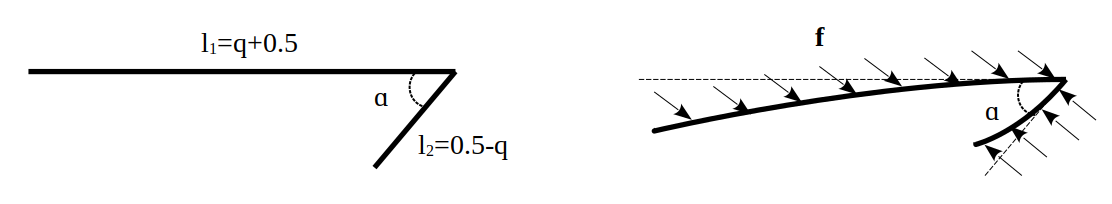
\includegraphics[width=1\textwidth]{plot/geometry.png}
		\caption{Schematics of the geometry of the boomerang. The left diagram illustrates the case without any applied force, while the right diagram shows a deformed configuration with traction $\mathbf{f}$ acting on it.}
		\label{fig:1}
	\end{center}
	%	\setlength{\abovecaptionskip}{-0.5 cm}
\end{figure}
Note that there are several extreme cases:
\begin{equation}
	\label{eqn:1}
	\left.
	\begin{aligned}
		&\alpha=0,\pi \\
		&	q=0.5
	\end{aligned}
	\right\}\Longrightarrow \text{straight rod},\quad 
	q=0, \alpha \neq 0, \pi \Longrightarrow \text{same arm length}.
\end{equation}
We exclude the case where the object becomes a straight rod (considering the ranges of $q$ and $\alpha$), as this shape yields only the trivial solution by using slender body theory. We assume that the boomerang has a small radius $\frac{h}{2}\ll \min\{l_1, l_2\}$, and define the aspect ratio $\epsilon$, which is small, such that $\epsilon=\frac{h/2}{\min\{l_1, l_2\}}\ll1$. 

\begin{figure}[!h]
	\begin{center}
		% specify width as 80% of the width of the text on the page
		% we can also specify a width in centimetres, e.g. [width=8cm]
		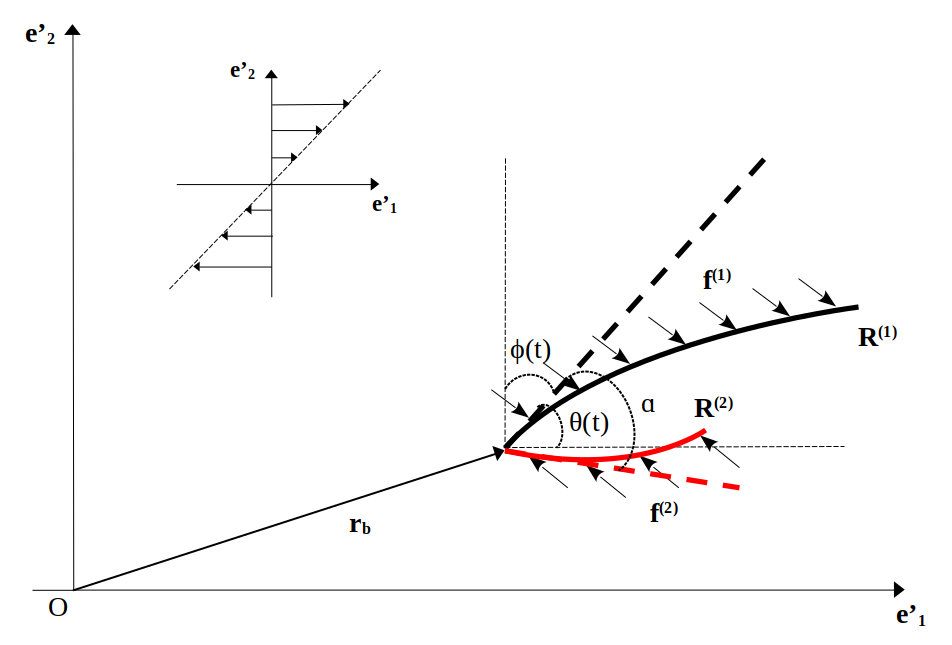
\includegraphics[width=0.8\textwidth]{plot/fluid.png}
		\caption{Schematic of an elastic boomerang-shaped fibre in the deformed state immersed in shear flow. The dashed black and dashed red lines represent the undeformed configurations corresponding to the deformed arms $\mathbf{R}^{(1)}$ and $\mathbf{R}^{(2)}$, respectively. $\alpha$ is the opening angle between the two dashed lines.} 
		\label{fig:6}
	\end{center}
	%	\setlength{\abovecaptionskip}{-0.5 cm}
\end{figure}
\begin{figure}[htb]
	\begin{center}
		% specify width as 80% of the width of the text on the page
		% we can also specify a width in centimetres, e.g. [width=8cm]
		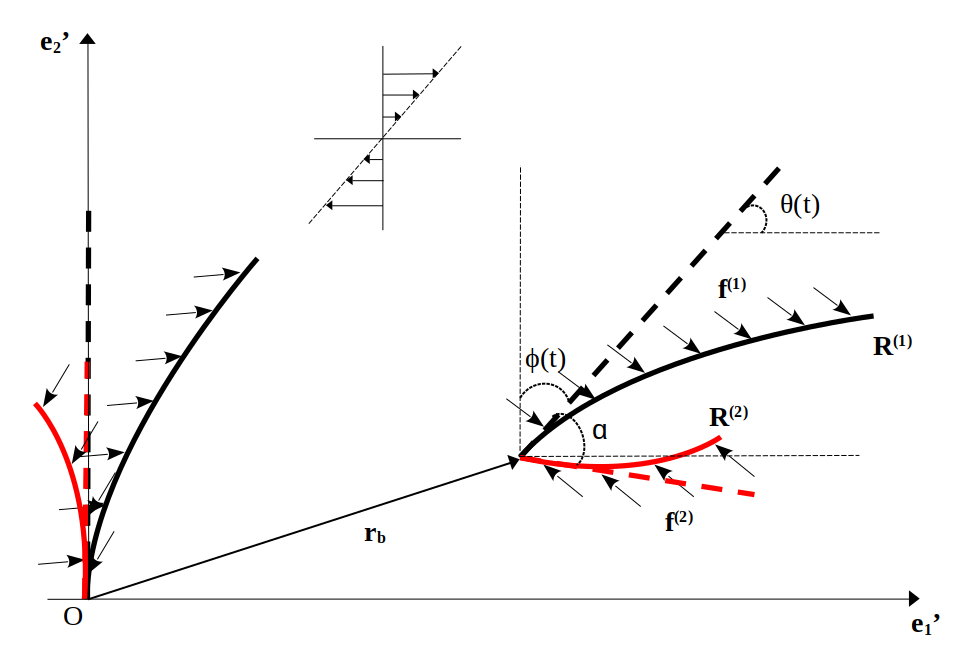
\includegraphics[width=0.8\textwidth]{plot/elastic_case/deformed_config.png}
		\caption{Schematic of an elastic boomerang-shaped fibre in the deformed state immersed in shear flow. The dashed black and dashed red lines represent the undeformed configurations corresponding to the deformed arms $\mathbf{R}^{(1)}$ and $\mathbf{R}^{(2)}$, respectively. $\alpha$ is the opening angle between the two dashed lines.}
		\label{fig:22}
	\end{center}
	%	\setlength{\abovecaptionskip}{-0.5 cm}
\end{figure}
To implement the algorithm for this fibre, we model it as two elastic beams joined at the hinge point. Initially, both beams are clamped at the origin, differing in length and rotation angle. The length of the long beam is $q+0.5$, while the short beam's length is $0.5-q$, where $q \in [0,0.5)$. The rotation angle for the long beam is given by the inclination $\phi(t)$, whereas for the short beam, it is $\phi(t)+\alpha$. Figure \ref{fig:6} provides a schematic illustration of this process. 


\subsection{Equilibrium solutions}
\subsubsection{Four equilibria}
Roggeveen and Stone have studied the dynamics of this fibre shape for the rigid case, namely $\mathcal{I}=0$, in shear flow at zero Reynolds number. If, when $\mathcal{I}=0$, the solutions coincide with the results presented in their paper, it would lend a certain degree of validation to our results.
We run multiple examples using \texttt{oomph-lib} and select some representative cases to present in this report. Similar to the results of Roggeveen and Stone in Figure \ref{fig:18}, the complete solutions of the system also exhibit four equilibria. Of these four fixed orientations, two differ from the other two by an angle of $\pi$ but possess the same shapes, as shown in Figure \ref{fig:20}. Hence, to simplify the discussion, we will focus solely on one group of the two solutions in the following sections.
\begin{figure}[!h]
	\begin{center}
		% specify width as 80% of the width of the text on the page
		% we can also specify a width in centimetres, e.g. [width=8cm]
		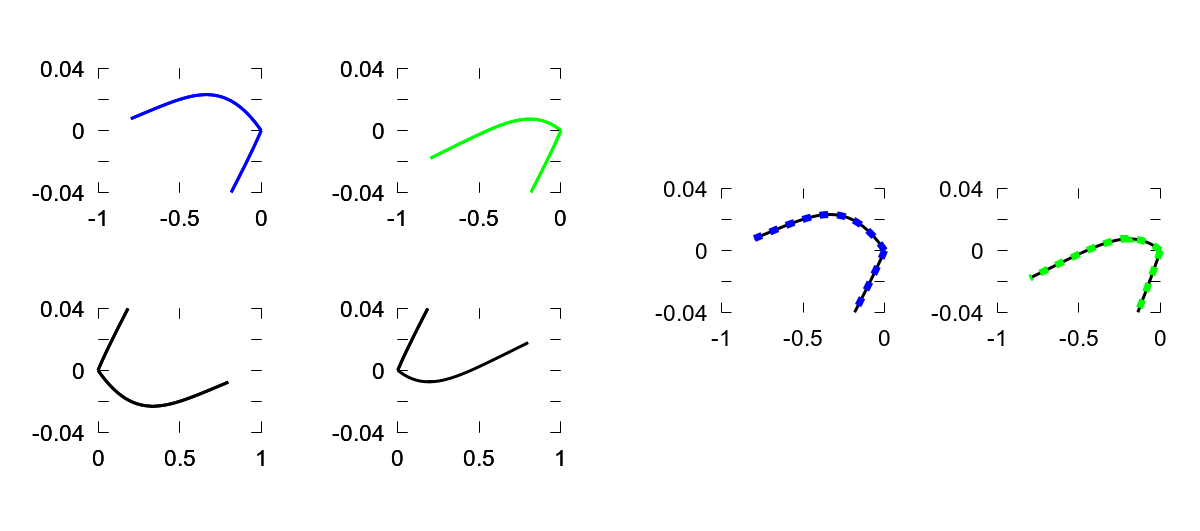
\includegraphics[width=1\textwidth]{plot/four_solutions2.png}
		\caption{Left: the complete solutions of the system for $q=0.3, \alpha=0.125\pi, \mathcal{I}=0.0003$. Right: the shapes are compared by rotating the black curve by $\pi$ to match the corresponding blue or green curve.}
		\label{fig:20}
	\end{center}
	%	\setlength{\abovecaptionskip}{-0.5 cm}
\end{figure}

\subsubsection{Effect of increasing FSI parameter $\mathcal{I}$}
We believe that plotting the steady orientation $\theta_{eq}$ against the FSI coefficient $\mathcal{I}$ could be an effective way to initially visualise the data. Figure \ref{fig:7} illustrates the case of $q = 0.4$ and $\alpha = 0.230\pi$. The curve begins and ends at $\mathcal{I}=0$, which is consistent with the rigid case results in Roggeveen and Stone's paper. To intuitively demonstrate the different deformations along the curve, we also attach the shapes of the particle at various points. There is a limit point within this curve where the deformed shapes on both the upper and lower branches converge and align with each other. We observe that the long arm undergoes more noticeable deformation, while the short arm shows no significant deformation. The deformed shapes can be classified by the number of humps in the deformed long arm. In Figure \ref{fig:7}, these shapes fall into the 'one hump' category.
\begin{figure}[!h]
	\begin{center}
		% specify width as 80% of the width of the text on the page
		% we can also specify a width in centimetres, e.g. [width=8cm]
		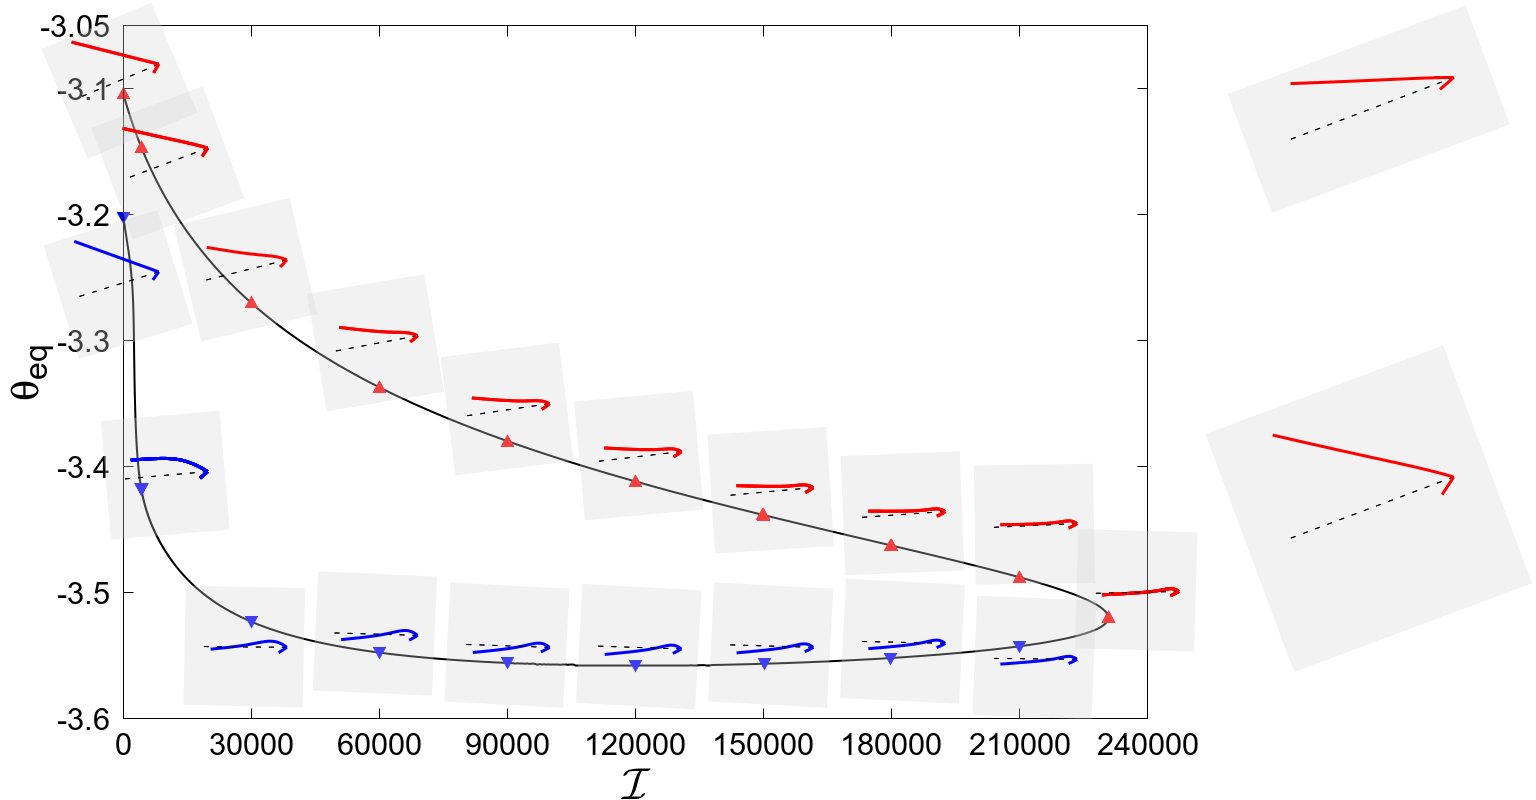
\includegraphics[width=1\textwidth]{plot/RESLT_q_0.40_alpha_0.230pi_plot_step_refine2_new_recale_FSI/combine_elastic_beam_I_theta_q_0.40_alpha_0.230pi_initial_-4.80_refine2_15_new.png}
		\caption{The steady orientation $\theta_{eq}$ is plotted against the FSI parameter $\mathcal{I}$ for the fibre with shape parameters $q = 0.4$ and $\alpha = 0.230\pi$. Deformations of all shapes are shown exaggeratedly. On the right-hand side, a comparison between the exaggerated and actual shapes is provided at a red point corresponding to $\mathcal{I}=3600$, to illustrate the scale of deformation. Thin black dashed line is the bisector of the opening angle $\alpha$, which is vertical to the right side of the grey blocks. Shapes are stretched by a factor of two along this side to make the deformations more apparent. Shapes along each branch of the curve consistently display the same colour. At the limit point, two branches coalesce and their corresponding fibre shapes become identical.}
		\label{fig:7}
	\end{center}
	%	\setlength{\abovecaptionskip}{-0.5 cm}
\end{figure}
Figure \ref{fig:8} depicts a more complex curve than Figure \ref{fig:7}, featuring numerous twists and additional limit points. The only difference in the initial undeformed shapes between this case and that of Figure \ref{fig:7} lies in the opening angle $\alpha$ between two arms: here, the opening angle is smaller than the previous case. This curve also begins and ends at $\mathcal{I}=0$, consistent with the rigid results. The shapes along the different branches ultimately align at the limit points. The outer branch of the curve is similar to Figure $\ref{fig:7}$'s case, with shapes in this branch also falling into the 'one hump' category. New shapes appear in the inner curve, where a tail develops at the end of the long arm. These shapes can be classified into the 'two humps' category. We also find that, compared to the previous case, $\mathcal{I}_{max}$ increases and $\theta_{eq,min}$ decreases. Additionally, a bifurcation occurs along the curve, revealing an even more intriguing phenomenon as $\alpha$ varies, as shown in Figure \ref{fig:9}.
\begin{figure}[!h]
	\begin{center}
		% specify width as 80% of the width of the text on the page
		% we can also specify a width in centimetres, e.g. [width=8cm]
		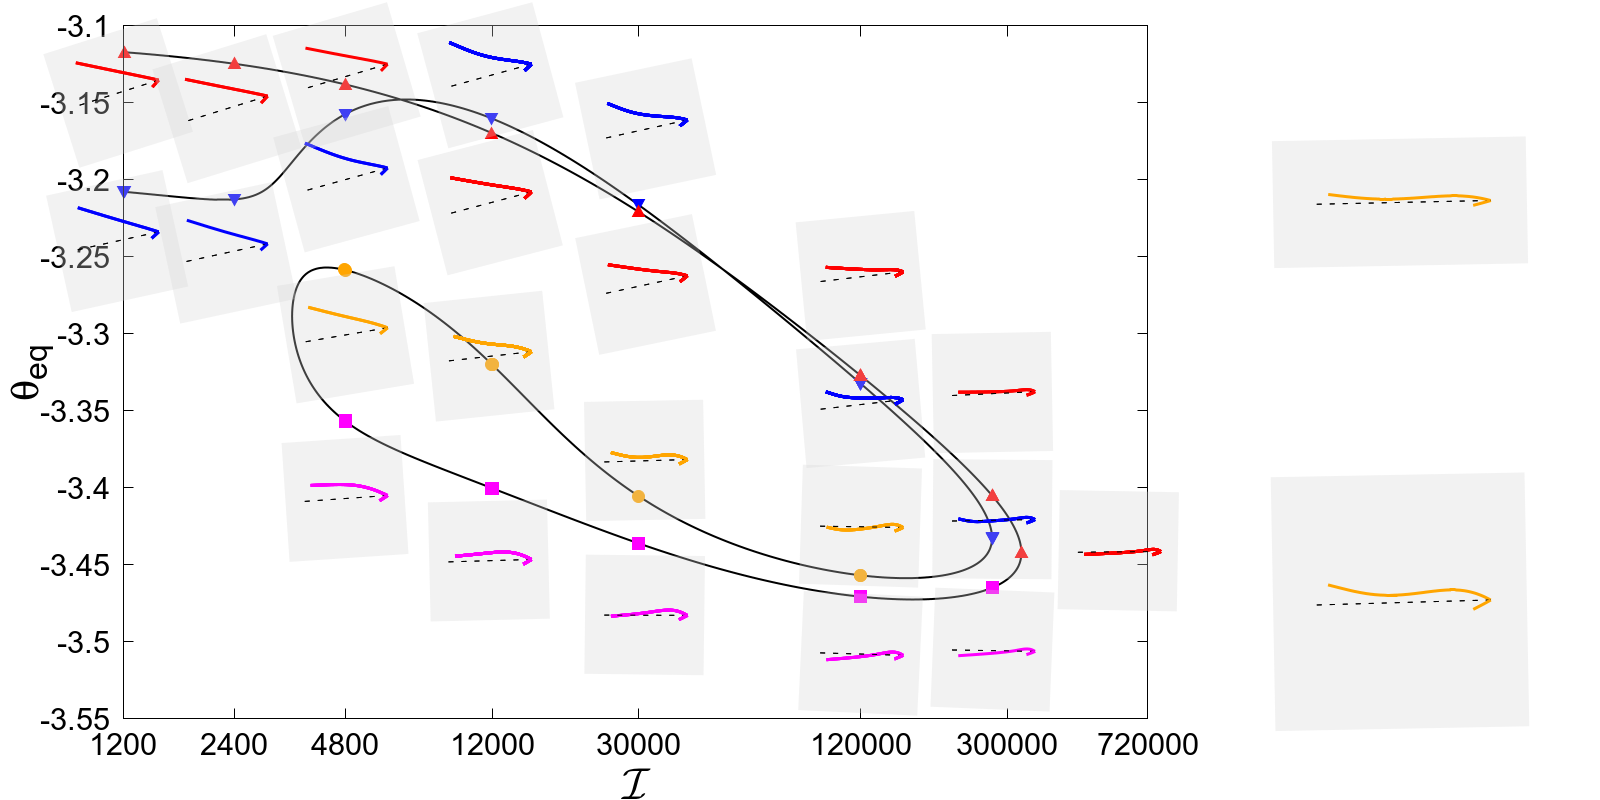
\includegraphics[width=1\textwidth]{plot/RESLT_q_0.40_alpha_0.180pi_plot_step_refine2_new_recale_FSI/combine_elastic_beam_I_theta_q_0.400_alpha_0.180pi_initial_-4.80_refine2_rescale_FSI.png}
		\caption{The steady orientation $\theta_{eq}$ is plotted against the FSI parameter $\mathcal{I}$ for the fibre with shape parameters $q = 0.4$ and $\alpha = 0.180\pi$. The shapes along the curve are also stretched by a factor of two along the right side of the grey block. Multiple limit points are observed along the curve, and a new type of deformation emerges, as shown on the right-hand side.}
		\label{fig:8}
	\end{center}
	%	\setlength{\abovecaptionskip}{-0.5 cm}
\end{figure}

Figure \ref{fig:9} is a sequence of logarithmic plots illustrating the bifurcation process as $\alpha$ increases. In the first three subplots, where $\alpha=0.180\pi,0.190\pi,0.200\pi$, the curve exhibits two prominent protrusions. As $\alpha$ increases, the distance between these protrusions gradually decreases. When $\alpha$ reaches a value between $0.200\pi$ and $0.210\pi$, a bifurcation occurs, giving rise to a new, independent inner closed loop (blue). This bifurcation signifies a critical transition in the system’s behaviour, where the previously connected equilibrium solutions split, leading to multiple distinct solution curves. We also check the shapes along the newly appeared blue curve still follow the observed pattern and belong to the 'two humps' category.
\begin{figure}[!h]
	\begin{center}
		% specify width as 80% of the width of the text on the page
		% we can also specify a width in centimetres, e.g. [width=8cm]
		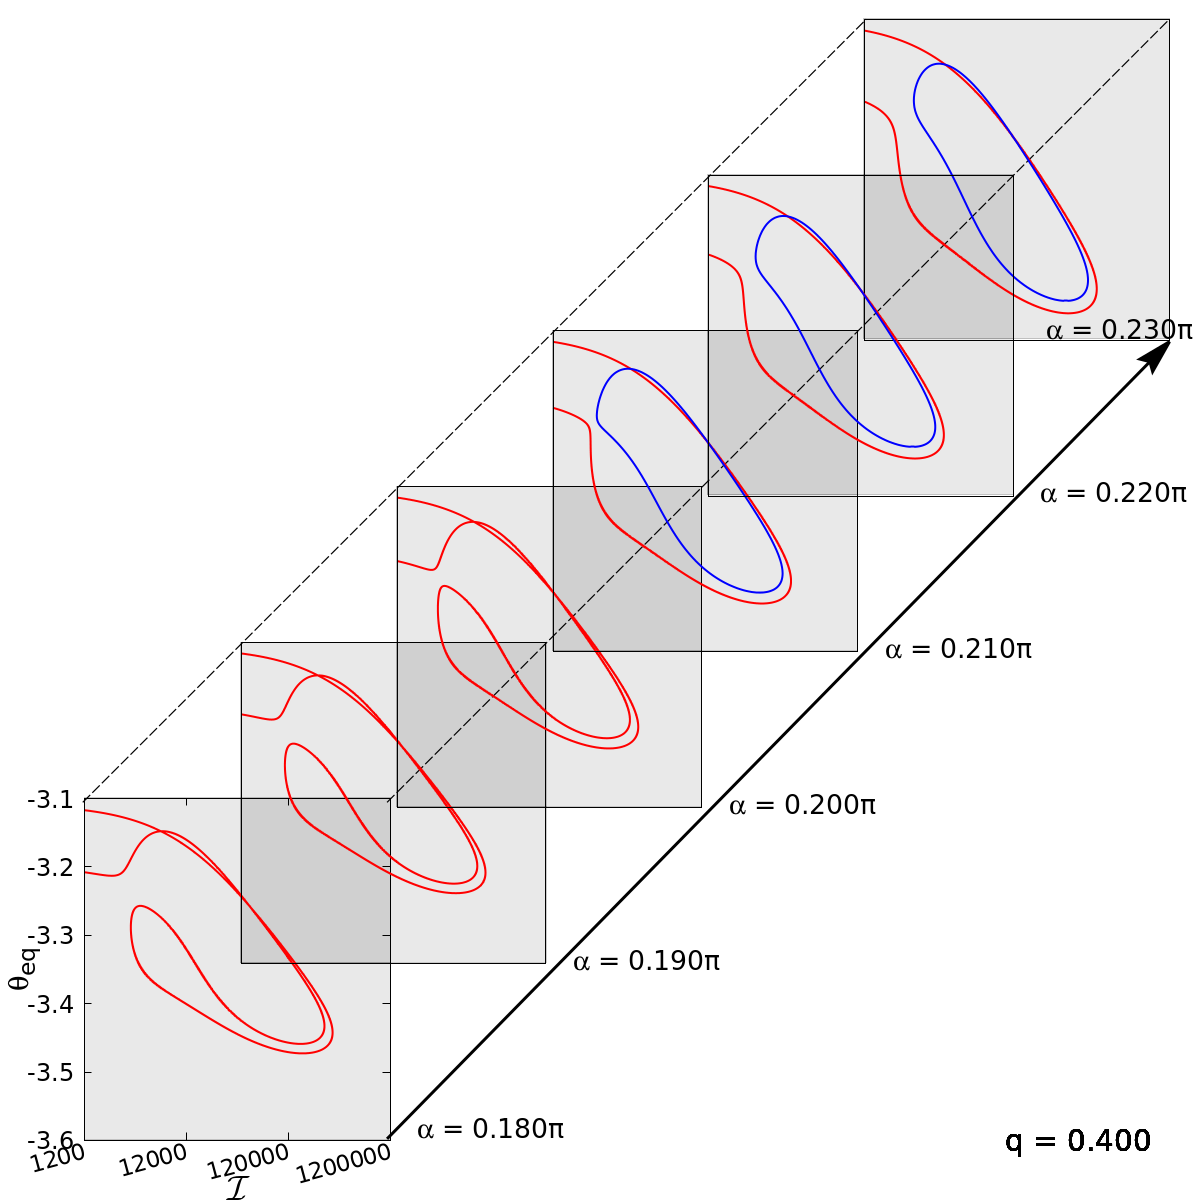
\includegraphics[width=0.7\textwidth]{plot/RESLT_animation_varying_alpha_q_0.400_step_rescale_FSI/elastic_beam_I_theta_q_0.400_alpha_5.png}
		\caption{A sequence of plots presents the steady orientation $\theta_{eq}$ against the FSI parameter $\mathcal{I}$ for shape parameters $q = 0.4$ with varying $\alpha$. The scale of the axes is consistent across all subplots.}
		\label{fig:9}
	\end{center}
	%	\setlength{\abovecaptionskip}{-0.5 cm}
\end{figure}
We find even more complex curves, and Figure \ref{fig:12} illustrates a representative case for a larger $q$, where the length of the short arm is very small. Although this curve appears complex, it still starts and ends at $\mathcal{I}=0$, maintaining consistency with the Roggeveen and Stone's results. The curve exhibits more twists and includes additional shape types. Intuitively, there are two new categories with corresponding new branches. In the outer new branch, the shapes (orange and dark blue) display 'three humps'. In the inner new branch, the shapes (dark green and brown) exhibit 'four humps,' with a tail forming at the end of the long arm, following the previous pattern where a tail appears in the shape on the inner branch of the curve. The two outermost branches, which are very close to each other, exhibit multiple intersections. This is why the order of the shapes (green and blue, cyan and purple) changes along these branches. The shapes along these two outermost branches still belong to the 'two humps' and 'one hump' categories. Actually, this complex curve has more bifurcations, as shown in Figure \ref{fig:13}.
\begin{figure}[!h]
	\begin{center}
		% specify width as 80% of the width of the text on the page
		% we can also specify a width in centimetres, e.g. [width=8cm]
		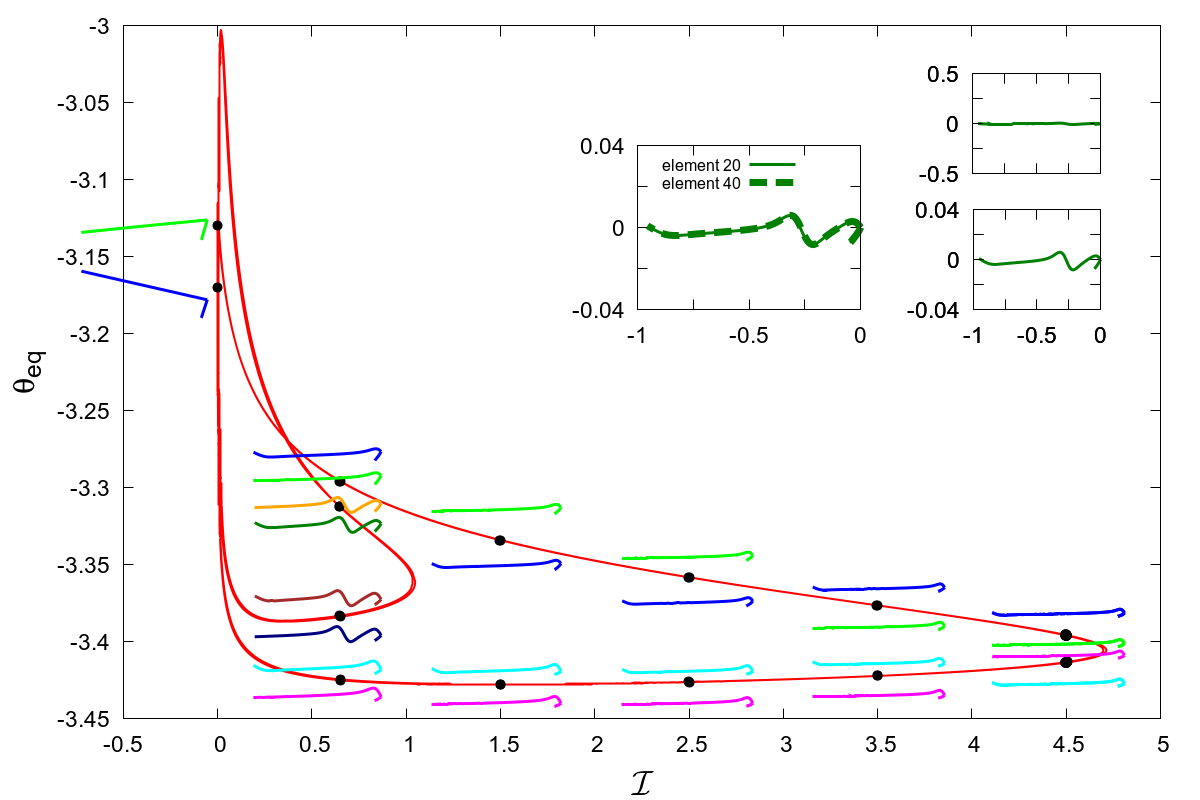
\includegraphics[width=1\textwidth]{plot/combine_elastic_beam_I_theta_q_0.452_alpha_0.125pi_initial_-4.80_0.png}
		\caption{The steady orientation $\theta_{eq}$ is plotted against the FSI coefficient $\mathcal{I}$ for the fibre with shape parameters $q = 0.452$ and $\alpha = 0.125\pi$. The top-right subplot shows the convergence test with doubled elements for the case at $\mathcal{I}=0.65$.}
		\label{fig:12}
	\end{center}
	%	\setlength{\abovecaptionskip}{-0.5 cm}
\end{figure}
\begin{figure}[!h]
	\begin{center}
		% specify width as 80% of the width of the text on the page
		% we can also specify a width in centimetres, e.g. [width=8cm]
		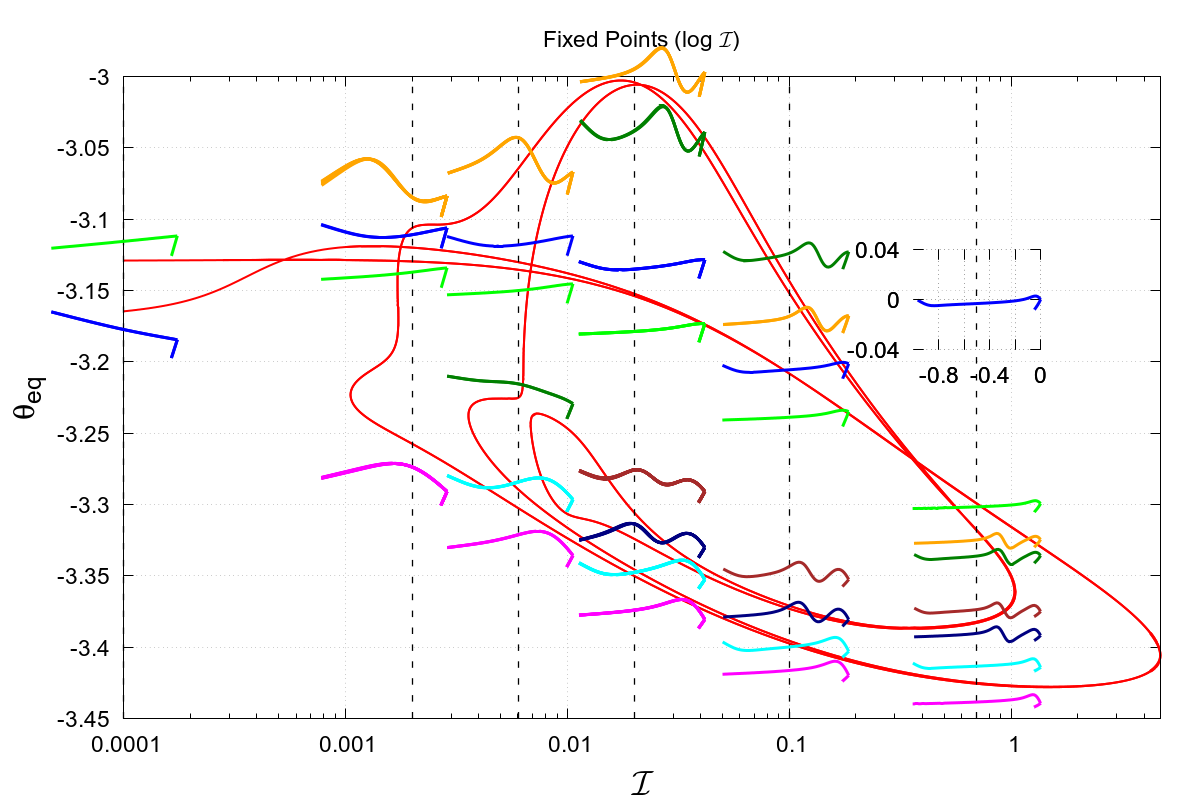
\includegraphics[width=1\textwidth]{plot/logx_combine_elastic_beam_I_theta_q_0.452_alpha_0.125pi_initial_-4.80_0.png}
		\caption{The steady orientation $\theta_{eq}$ is plotted against the FSI coefficient $\mathcal{I}$ for the fibre with shape parameters $q = 0.452$ and $\alpha = 0.125\pi$.}
	\end{center}
	%	\setlength{\abovecaptionskip}{-0.5 cm}
\end{figure}
\begin{figure}[!h]
	\centering
	\begin{minipage}{\linewidth}
		\centering
		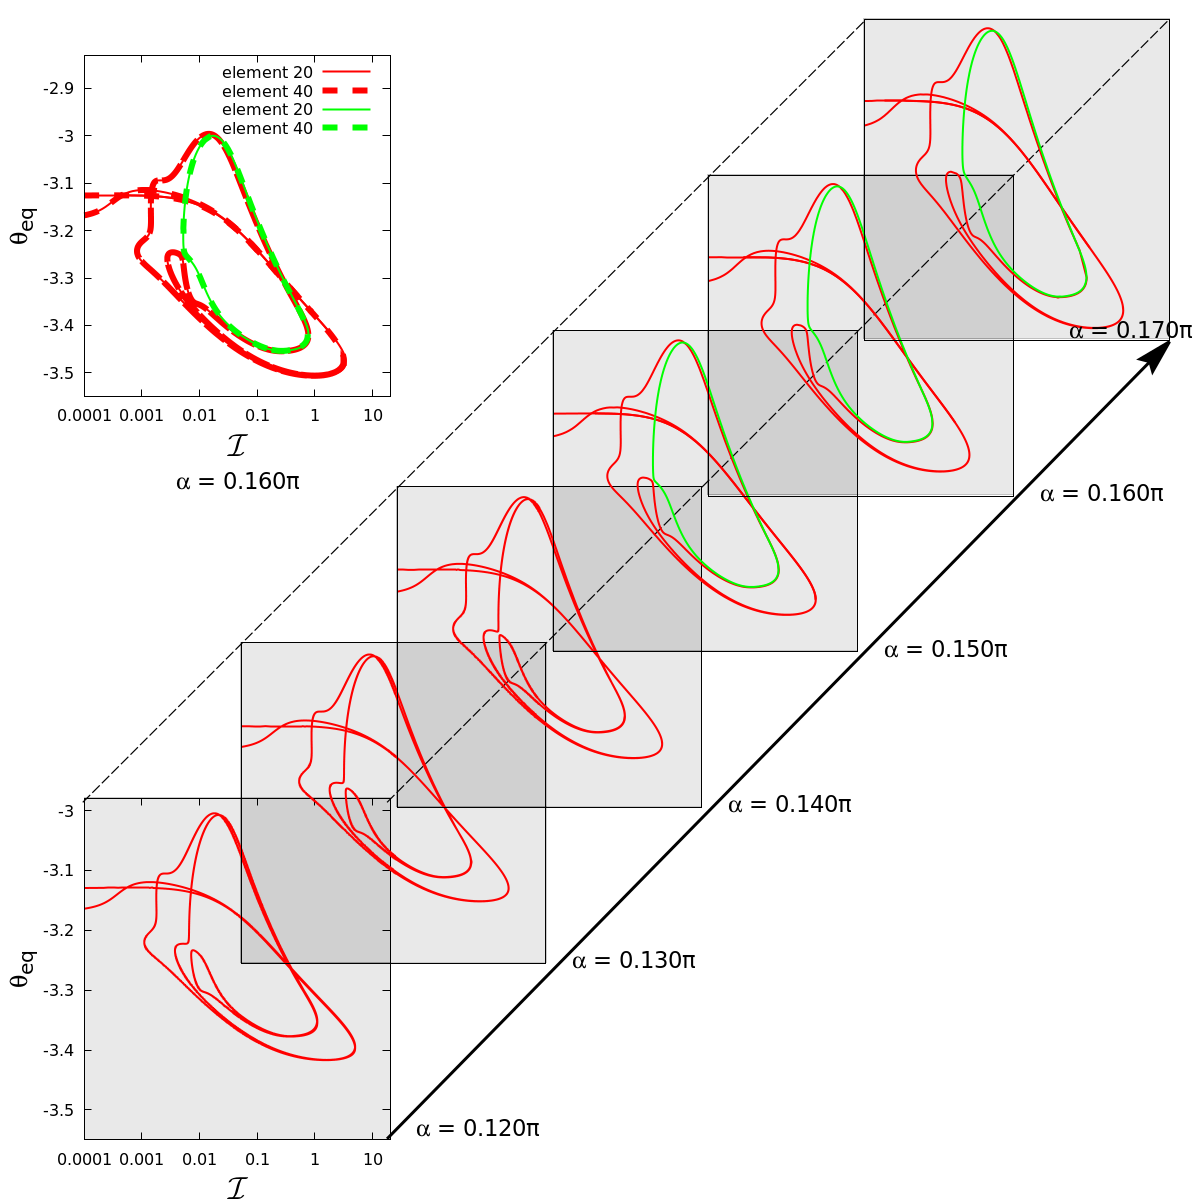
\includegraphics[scale=0.15]{plot/elastic_beam_I_theta_q_0.452_alpha_restart1.png}
	\end{minipage}
	\begin{minipage}{\linewidth}
		\centering
		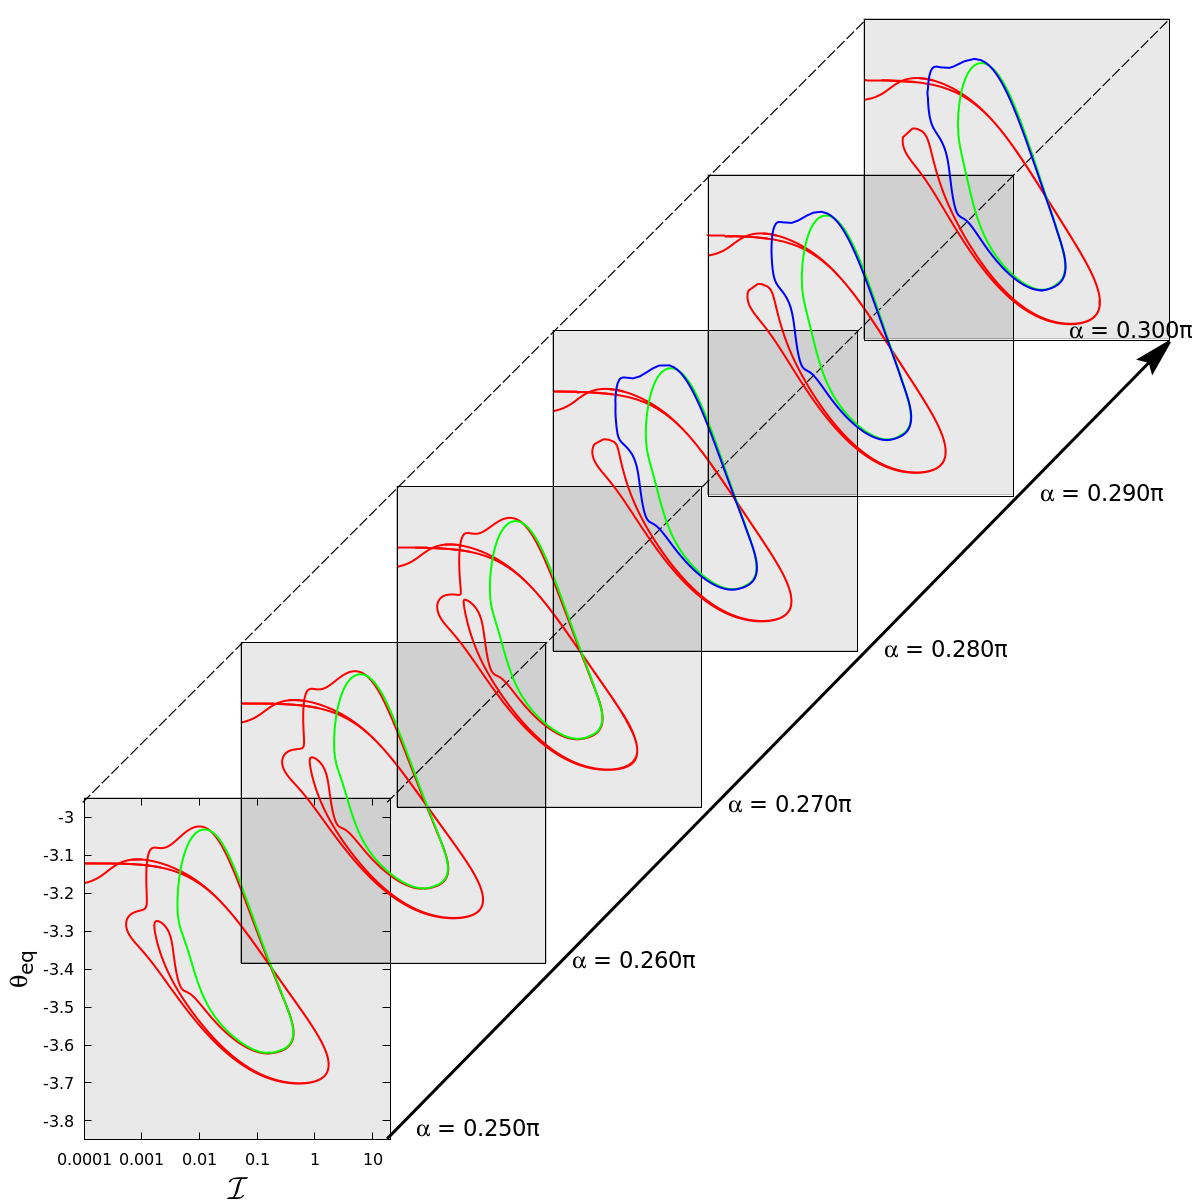
\includegraphics[scale=0.15]{plot/elastic_beam_I_theta_q_0.452_alpha_restart2.png}
	\end{minipage}
	\begin{minipage}{\linewidth}
		\centering
		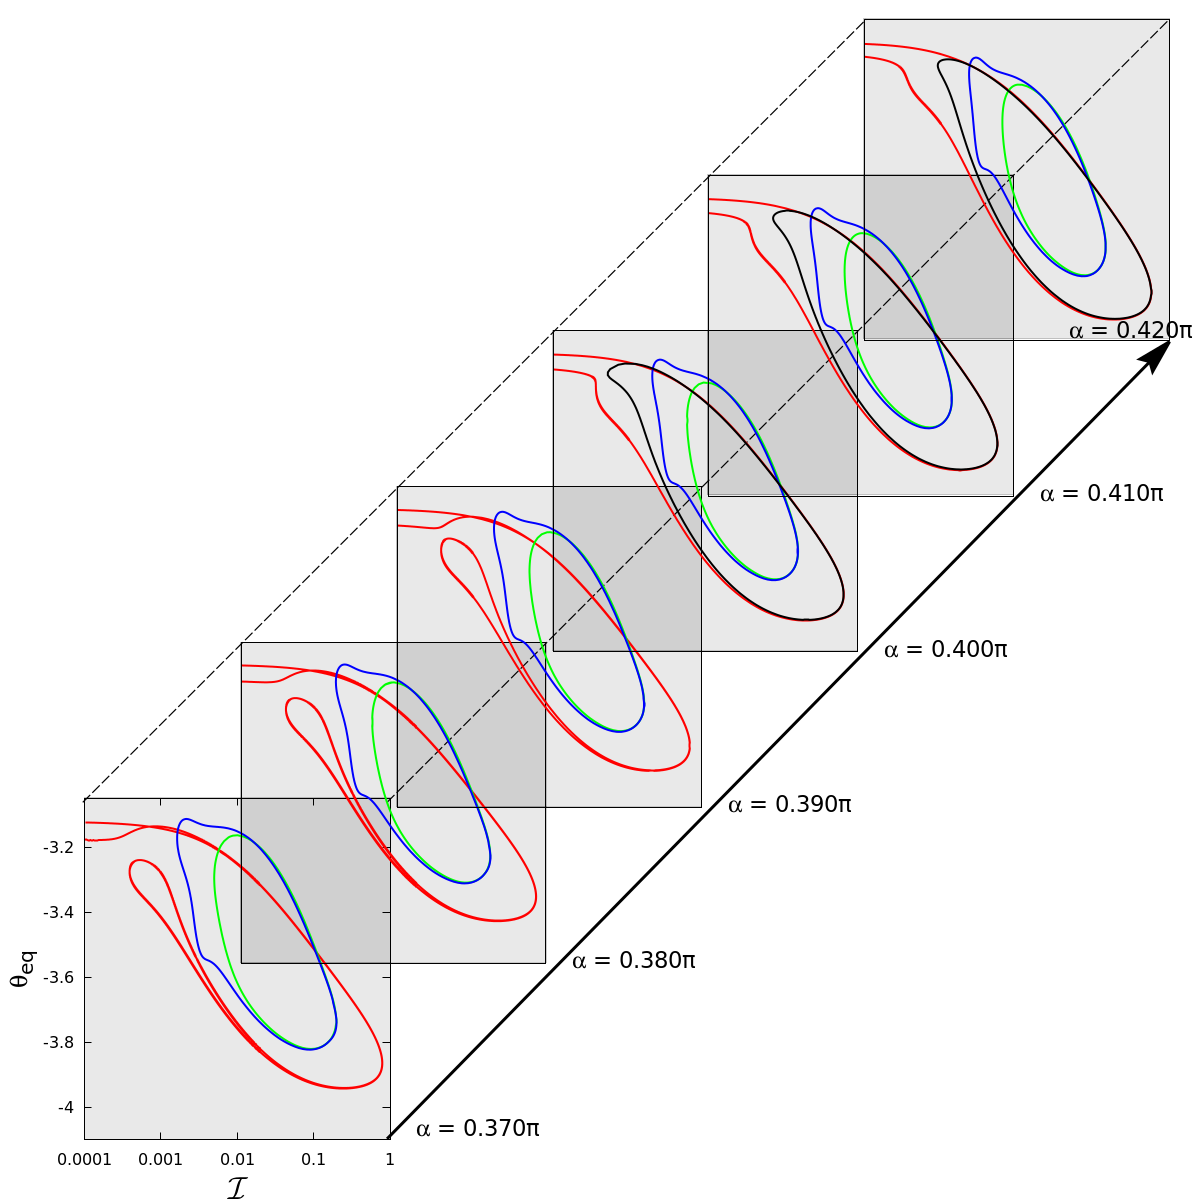
\includegraphics[scale=0.15]{plot/elastic_beam_I_theta_q_0.452_alpha_restart3.png}
	\end{minipage}
	\caption{A sequence of logarithmic plots presents the steady orientation $\theta_{eq}$ against the FSI coefficient $\mathcal{I}$ for shape parameters $q = 0.452$ with varying $\alpha$. The top-left subplot shows the convergence test with doubled elements, and the scale of the axes is consistent across all subplots.}
	\label{fig:13}
\end{figure}
In Figure \ref{fig:13}, there are three bifurcations as $\alpha$ varies, and we have selected three sequences to illustrate them. The explanations are generally similar: as $\alpha$ increases, two distinct protrusions gradually approach each other until they meet at a bifurcation point, causing the curve to split and generate a new independent closed loop. Subsequently, as $\alpha$ continues to increase, this new independent closed loop moves away from the previously connected curve. Finally, the curve splits into three inner closed loops (green, blue and black) and an outermost curve (red) that still connects to the two points at $\mathcal{I} = 0$. Note that after $\alpha=0.4\pi$, the four curves (three inner closed loops and one outermost curve) are independent with each other.

\subsubsection{$q-\alpha$ plot for different $\mathcal{I}$}
 Similarly to the Roggeveen and Stone's $q-\alpha$ plot in Figure \ref{fig:18}, we aim to determine the boundary of the region where steady orientations exist for the elastic fibre case. To achieve this, we first plot the steady orientation $\theta_{eq}$ against the opening angle $\alpha$, as shown in Figure \ref{fig:14}. 
 \begin{figure}[!h]
	\begin{center}
		% specify width as 80% of the width of the text on the page
		% we can also specify a width in centimetres, e.g. [width=8cm]
		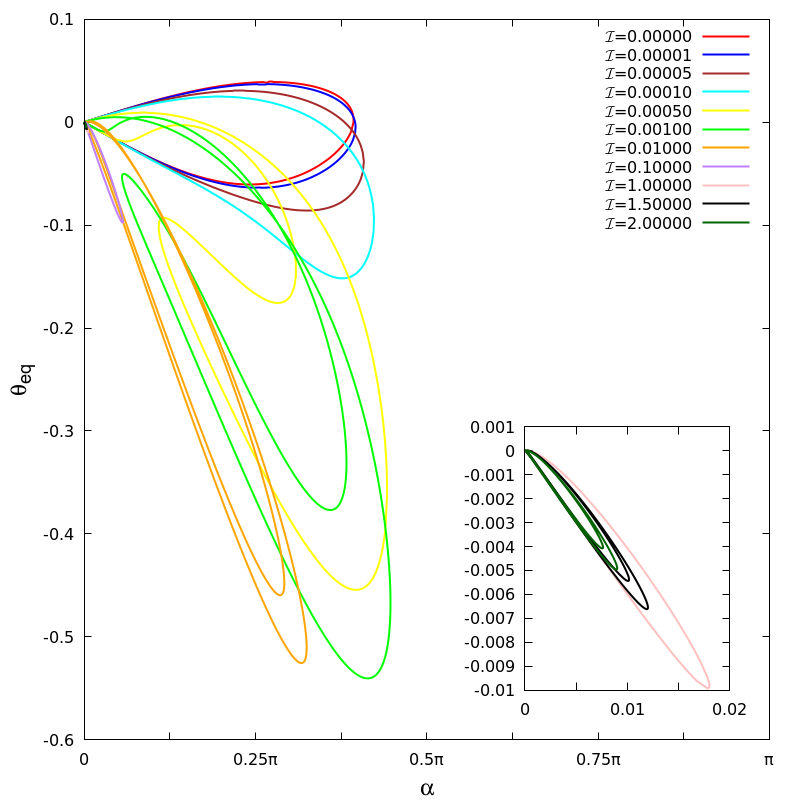
\includegraphics[width=0.6\textwidth]{plot/elastic_beam_alpha_theta_eq_q_0.400.png}
		\caption{The steady orientation $\theta_{eq}$ is plotted against  the opening angle $\alpha$ for the fibre with $q = 0.4$. The bottom-right subplot shows the figures of $\mathcal{I}=1.0, 1.5, 2.0$ at a smaller scale.}
		\label{fig:14}
	\end{center}
	%	\setlength{\abovecaptionskip}{-0.5 cm}
\end{figure}
In Figure \ref{fig:14}, as $\mathcal{I}$ increases, $\alpha_{max}$ initially rises and then rapidly decreases. We observe that every curve for different values of $\mathcal{I}$ forms a closed loop. Therefore, by tracing $\alpha_{max}$ for various $\mathcal{I}$, we can determine the boundary of the steady orientation region. Figure \ref{fig:15} shows the boundary we concern for different FSI coefficient $\mathcal{I}$. The red line represents the boundary for $\mathcal{I}=0$, which aligns with the results from Roggeveen and Stone's paper. Generally, as $\mathcal{I}$ increases, the region initially expands and then contracts. We can analyse this plot alongside Figure \ref{fig:14}. Focusing on a vertical line at $q = 0.4$, we observe that as $\mathcal{I}$ increases within the range $[0, 0.001]$ (from red to green), the boundary expands, indicating that $\alpha_{max}$ increases in Figure \ref{fig:15}. However, starting from  $\mathcal{I} = 0.01$ (orange), the region begins to shrink, meaning that $\alpha_{max}$ decreases in Figure \ref{fig:15}. It appears that there is a threshold around $\mathcal{I}=0.001$ (green). Before this threshold, as $\mathcal{I}$ increases, $\alpha_{max}$ also increases. After this point, when $\mathcal{I}$ increases, $\alpha_{max}$ decreases rapidly. In addition, we observe that when $\mathcal{I}\geq1$ (pink), the boundary reaches a relatively solid state. As the value of $\mathcal{I}$ increases, it appears that the boundary approaches its limit and changes more slowly.
\begin{figure}[!h]
	\begin{center}
		% specify width as 80% of the width of the text on the page
		% we can also specify a width in centimetres, e.g. [width=8cm]
		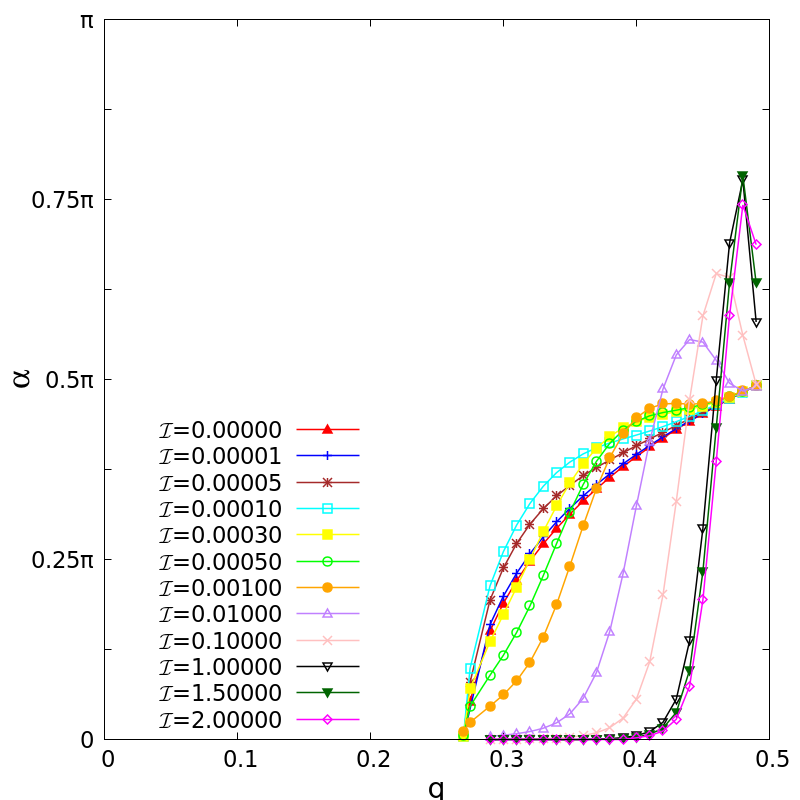
\includegraphics[width=0.6\textwidth]{plot/RESLT_q_alpha_plot/elastic_beam_general.png}
		\caption{This plot shows the boundary of the fixed points region for different FSI parameter $\mathcal{I}$.}
		\label{fig:15}
	\end{center}
	%	\setlength{\abovecaptionskip}{-0.5 cm}
\end{figure}
\begin{figure}[!h]
	\begin{center}
		% specify width as 80% of the width of the text on the page
		% we can also specify a width in centimetres, e.g. [width=8cm]
		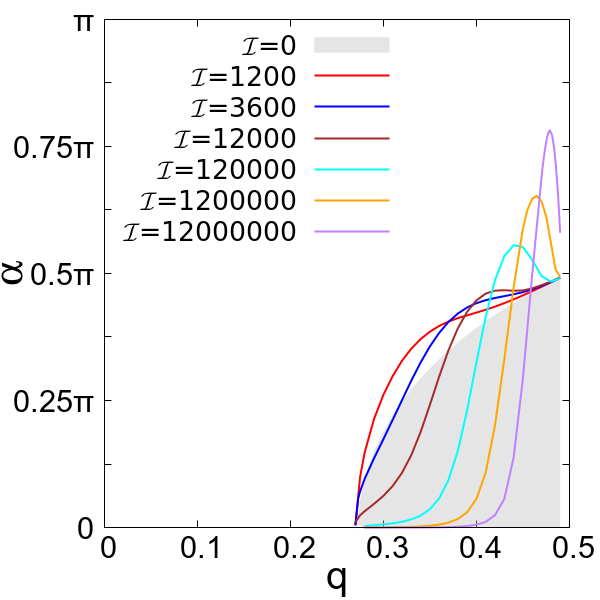
\includegraphics[width=0.6\textwidth]{plot/RESLT_q_alpha_plot_paper/elastic_beam_general.png}
		\caption{This plot shows the boundary of the steady orientation region for different FSI parameter $\mathcal{I}$.}
		\label{fig:26}
	\end{center}
	%	\setlength{\abovecaptionskip}{-0.5 cm}
\end{figure}


\subsubsection{Stability}
\begin{figure}[!h]
	\begin{center}
		% specify width as 80% of the width of the text on the page
		% we can also specify a width in centimetres, e.g. [width=8cm]
		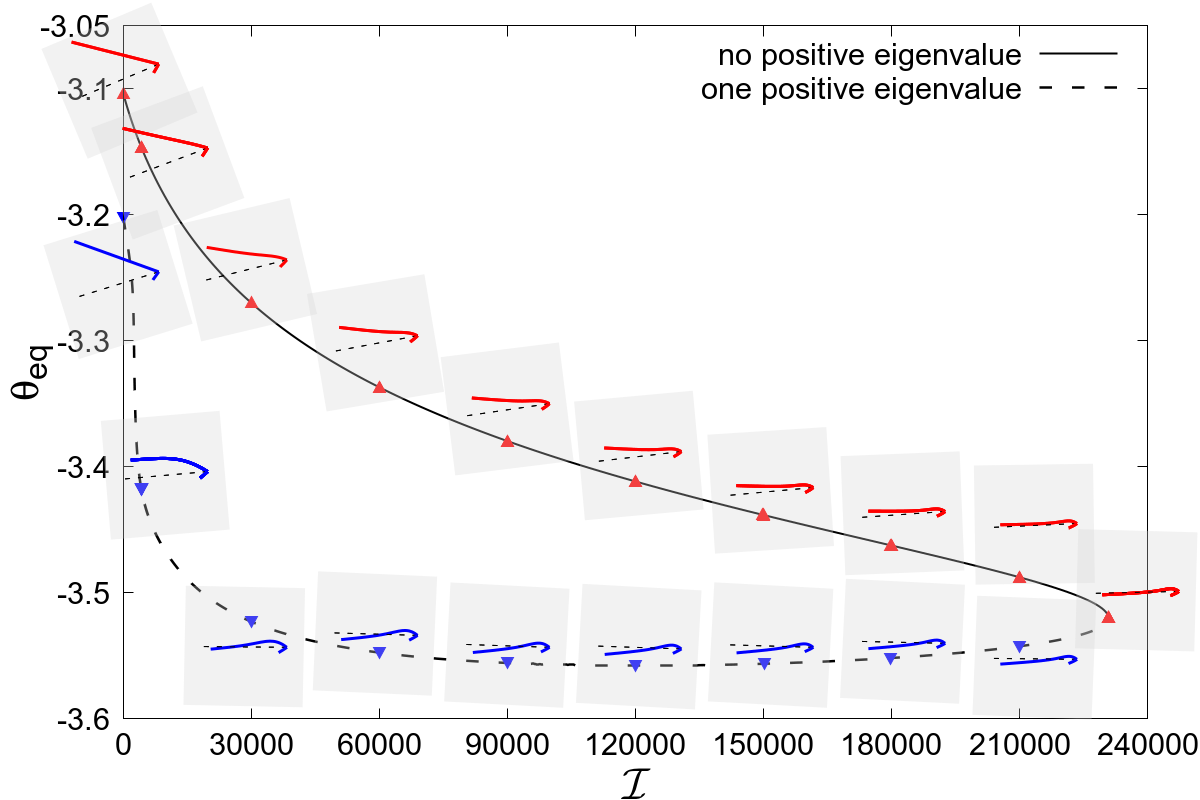
\includegraphics[width=0.8\textwidth]{plot/RESLT_q_0.40_alpha_0.230pi_plot_step_refine2_new_recale_FSI/combine_elastic_beam_I_theta_q_0.40_alpha_0.230pi_initial_-4.80_refine2_15_new_not_log_dash_line.png}
		\caption{The linear stability analysis for the case $q=0.4,\alpha=0.230\pi$ shows that there is no positive eigenvalue along the upper branch, indicating that the entire system is stable. After the limit point, a positive eigenvalue emerges, causing the lower branch unstable. This behaviour is consistent with the rigid case when $\mathcal{I}=0$, where the upper point is stable and the lower point is unstable.}
		\label{fig:10}
	\end{center}
	%	\setlength{\abovecaptionskip}{-0.5 cm}
\end{figure}
\begin{figure}[!h]
	\begin{center}
		% specify width as 80% of the width of the text on the page
		% we can also specify a width in centimetres, e.g. [width=8cm]
		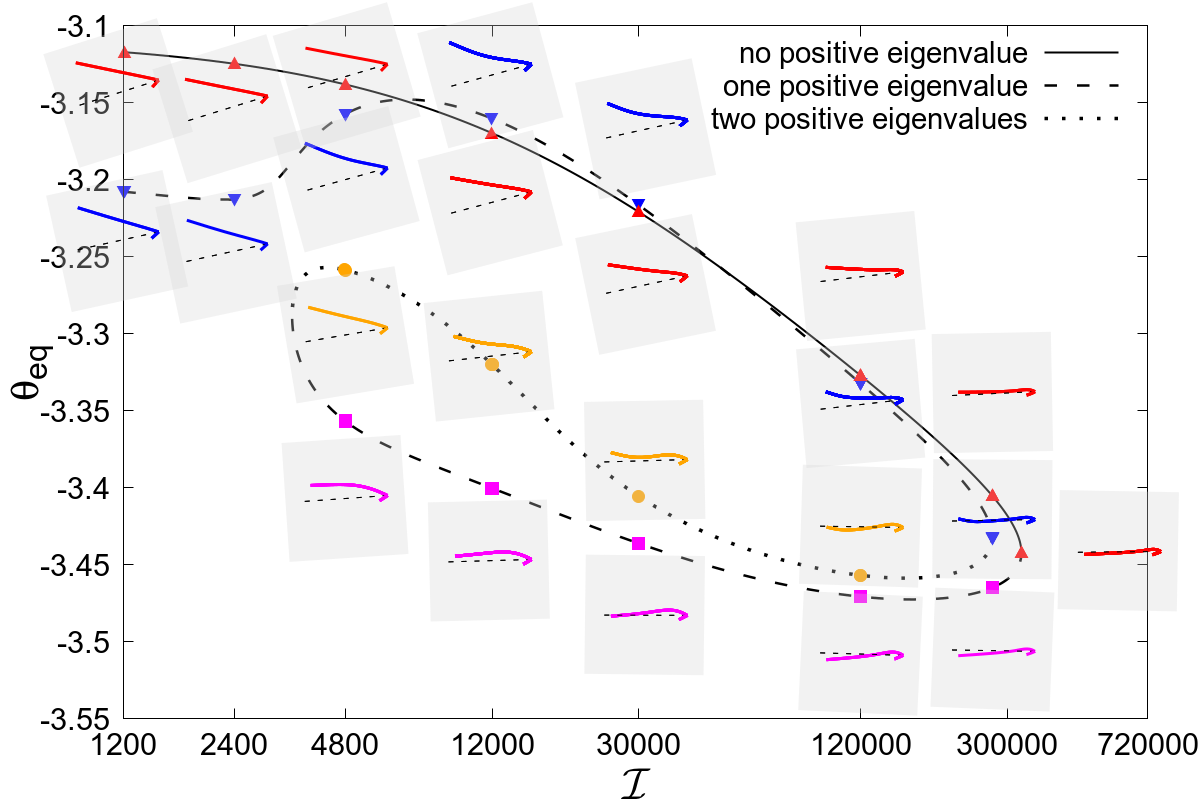
\includegraphics[width=0.8\textwidth]{plot/RESLT_q_0.40_alpha_0.180pi_plot_step_refine2_new_recale_FSI/combine_elastic_beam_I_theta_q_0.400_alpha_0.180pi_initial_-4.80_refine2_new_dash_line.png}
		\caption{The linear stability analysis for the case $q=0.4,\alpha=0.180\pi$ reveals a more complex scenario. The upper branch (solid line) remains stable, as no positive eigenvalues are present. After the rightmost limit point, the system becomes unstable with the emergence of a single positive eigenvalue (long-dashed line). Following the left limit point, the stability does not switch, but an additional positive eigenvalue appears (short-dashed line), resulting in two positive eigenvalues in total. Subsequently, at the right limit point, although the stability does not exchange, one of the positive eigenvalues vanishes (returning to the long-dashed line). These results remain consistent with the rigid case.}
		\label{fig:11}
	\end{center}
	%	\setlength{\abovecaptionskip}{-0.5 cm}
\end{figure}
\begin{figure}[!h]
	\begin{center}
		% specify width as 80% of the width of the text on the page
		% we can also specify a width in centimetres, e.g. [width=8cm]
		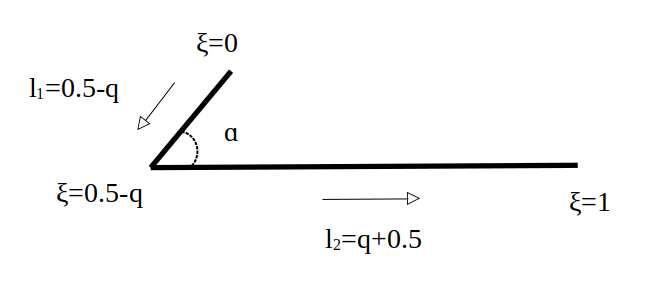
\includegraphics[width=0.5\textwidth]{plot/tensile_boomerang.png}
		\caption{The rigid structure fibre ($\mathcal{I}=0$).}
		\label{fig:16}
	\end{center}
	%	\setlength{\abovecaptionskip}{-0.5 cm}
\end{figure}

\newpage
To understand the mechanism of deformation, we define the tensile stress as 
\begin{equation}
	\label{eqn:91}
	\sigma(\xi)=\int_0^\xi (\mathbf{f}\cdot\mathbf{t}) \left |\frac{\partial \mathbf{R}}{\partial \xi}\right|\,d\xi,
\end{equation}
where $\mathbf{t}$ is the unit tangent vector to the surface of the fibre. As shown in Figure \ref{fig:15}, we use $\sigma_1$ and $\mathbf{t}_1$ to denote the tensile stress and tangent vector in the short arm, and $\sigma_2$ and $\mathbf{t}_2$ for the long arm. At the hinge point, we have 
\begin{equation}
	\label{eqn:92}
	\sigma_1(0.5-q)=\mathbf{F}_1\cdot\mathbf{t}_1, 
\end{equation}
\begin{equation}
	\label{eqn:93}
	\sigma_2(0.5-q)=\mathbf{F}_2\cdot\mathbf{t}_2, 
\end{equation}
where $\mathbf{F}_1$ and $\mathbf{F}_2$ represent the net drag acting on the short arm and long arm, respectively. Then, if $\xi \in [0,0.5-q]$, we have 
\begin{equation}
	\label{eqn:94}
	\sigma_1(\xi)= \int_0^\xi (\mathbf{f}\cdot\mathbf{t}_1) \left |\frac{\partial \mathbf{R}}{\partial \xi}\right|\,d\xi.
\end{equation}
If $\xi \in [0.5-q,1]$, we have
\begin{equation}
	\label{eqn:95}
	\begin{aligned}
		\sigma_2(\xi)&= \int_0^\xi (\mathbf{f}\cdot\mathbf{t}_2) \left |\frac{\partial \mathbf{R}}{\partial \xi}\right|\,d\xi\\
		&=\int_0^{0.5-q} (\mathbf{f}\cdot\mathbf{t}_2) \left |\frac{\partial \mathbf{R}}{\partial \xi}\right|\,d\xi+\int_{0.5-q}^\xi (\mathbf{f}\cdot\mathbf{t}_2) \left |\frac{\partial \mathbf{R}}{\partial \xi}\right|\,d\xi\\
		&=\mathbf{F}_1\cdot\mathbf{t}_2+\int_{0.5-q}^\xi (\mathbf{f}\cdot\mathbf{t}_2) \left |\frac{\partial \mathbf{R}}{\partial \xi}\right|\,d\xi.
	\end{aligned}
\end{equation}
Since we are investigating the equilibrium state, the components of the two net drag forces in the $\mathbf{t}_2$ direction must also be balanced. Hence, we have 
\begin{equation}
	\label{eqn:96}
	\mathbf{F}_1\cdot\mathbf{t}_2=-\mathbf{F}_2\cdot\mathbf{t}_2.
\end{equation}
Now, substituting \eqref{eqn:96} into the last step of \eqref{eqn:95}, we obtain 
\begin{equation}
	\begin{aligned}
		\label{eqn:97}
		\sigma_2(\xi)&=-\mathbf{F}_2\cdot\mathbf{t}_2+\int_{0.5-q}^\xi (\mathbf{f}\cdot\mathbf{t}_2) \left |\frac{\partial \mathbf{R}}{\partial \xi}\right|\,d\xi\\
		&=-\sigma_2(0.5-q)+\int_{0.5-q}^\xi (\mathbf{f}\cdot\mathbf{t}_2) \left |\frac{\partial \mathbf{R}}{\partial \xi}\right|\,d\xi.
	\end{aligned}
\end{equation}
Therefore, we have 
\begin{equation}
	\sigma(\xi)=\left\{
	\begin{aligned}
		\label{eqn:98}
		&\int_0^\xi (\mathbf{f}\cdot\mathbf{t}_1) \left |\frac{\partial \mathbf{R}}{\partial \xi}\right|\,d\xi,\quad \xi\in[0,0.5-q];\\
		&-\mathbf{F}_2\cdot\mathbf{t}_2+\int_{0.5-q}^\xi (\mathbf{f}\cdot\mathbf{t}_2) \left |\frac{\partial \mathbf{R}}{\partial \xi}\right|\,d\xi, \quad \xi\in[0.5-q,1].
	\end{aligned}\right.
\end{equation}
\begin{figure}[!h]
	\centering
	\subfigure[$q=0.35,\alpha=0.125\pi$]{
		\begin{minipage}[b]{0.3\textwidth}
			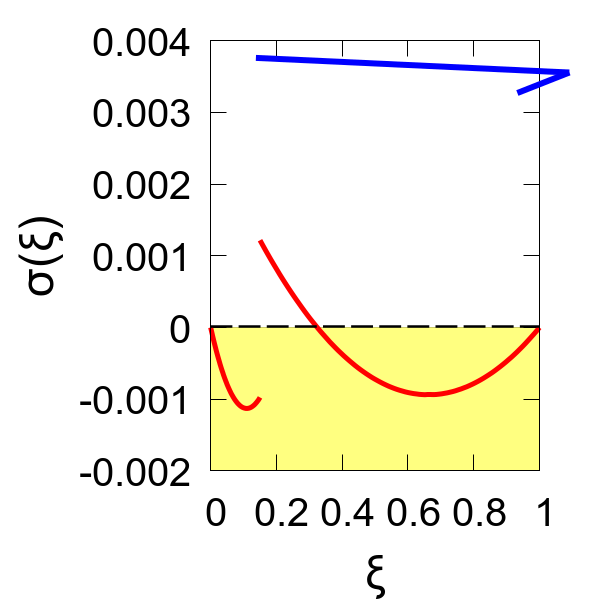
\includegraphics[width=1\textwidth]{plot/tensile_stress/sigma_q_0.35_alpha_0.125pi.png} 
		\end{minipage}
		\label{fig:16.a}
	}
	\subfigure[$q=0.40,\alpha=0.125\pi$]{
		\begin{minipage}[b]{0.3\textwidth}
			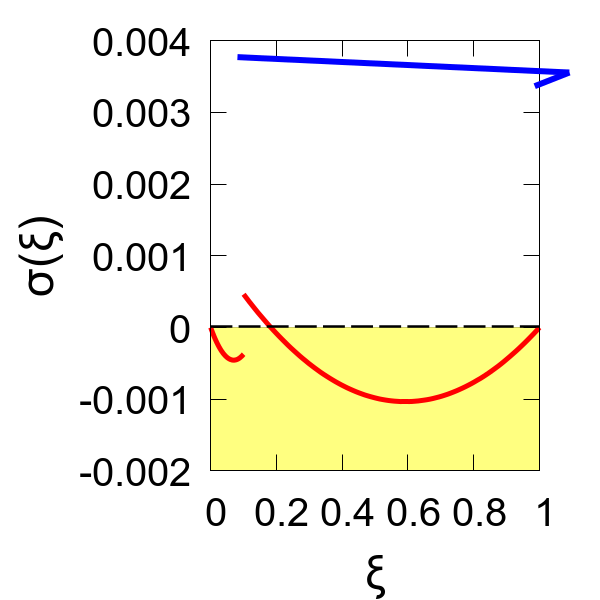
\includegraphics[width=1\textwidth]{plot/tensile_stress/sigma_q_0.40_alpha_0.125pi.png}
		\end{minipage}
		\label{fig:16.b}
	}
	\subfigure[$q=0.45,\alpha=0.125\pi$]{
		\begin{minipage}[b]{0.3\textwidth}
			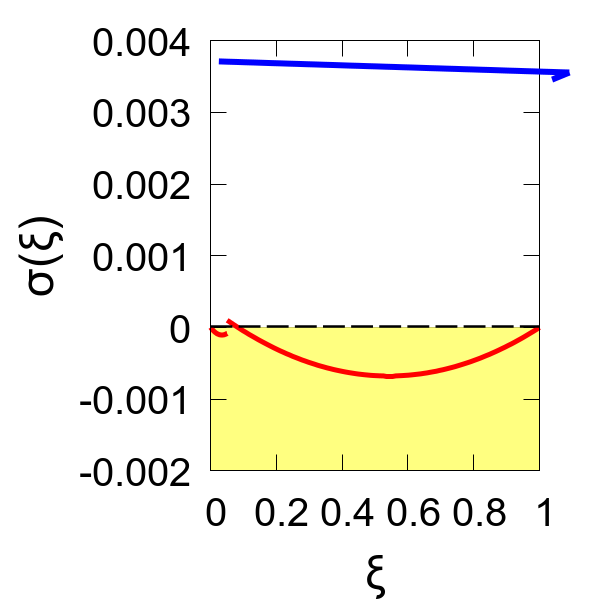
\includegraphics[width=1\textwidth]{plot/tensile_stress/sigma_q_0.45_alpha_0.125pi.png}
		\end{minipage}
		\label{fig:16.c}
	}
	\\ 
	\subfigure[$q=0.35,\alpha=0.25\pi$]{
		\begin{minipage}[b]{0.3\textwidth}
			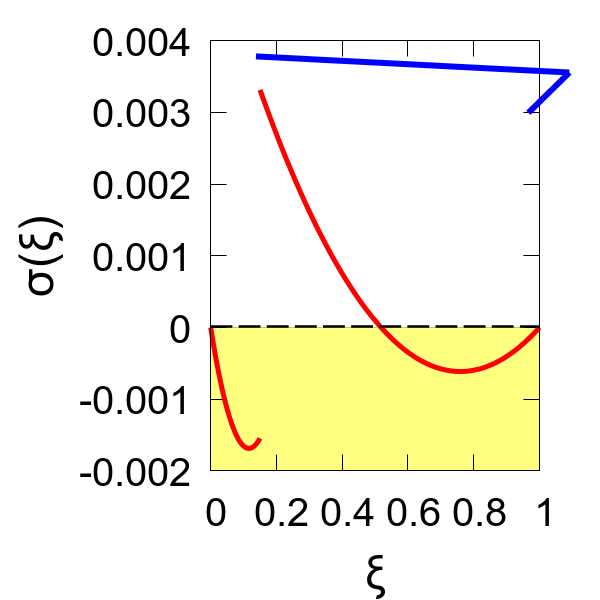
\includegraphics[width=1\textwidth]{plot/tensile_stress/sigma_q_0.35_alpha_0.250pi.png} 
		\end{minipage}
		\label{fig:16.d}
	}
	\subfigure[$q=0.40,\alpha=0.25\pi$]{
		\begin{minipage}[b]{0.3\textwidth}
			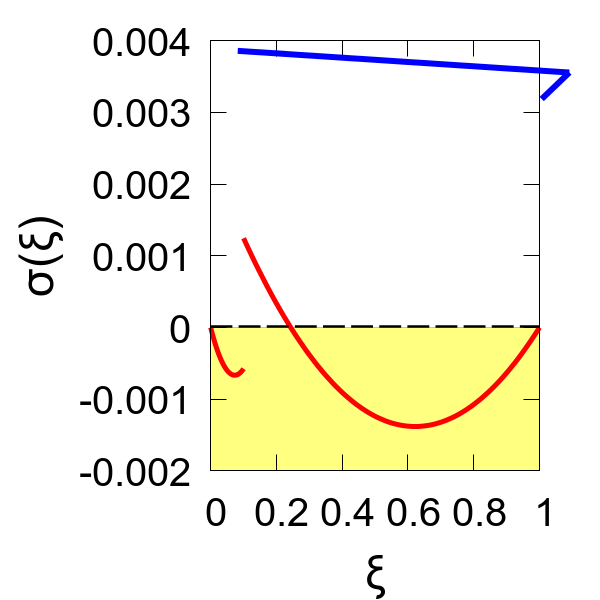
\includegraphics[width=1\textwidth]{plot/tensile_stress/sigma_q_0.40_alpha_0.250pi.png}
		\end{minipage}
		\label{fig:16.e}
	}
	\subfigure[$q=0.45,\alpha=0.25\pi$]{
		\begin{minipage}[b]{0.3\textwidth}
			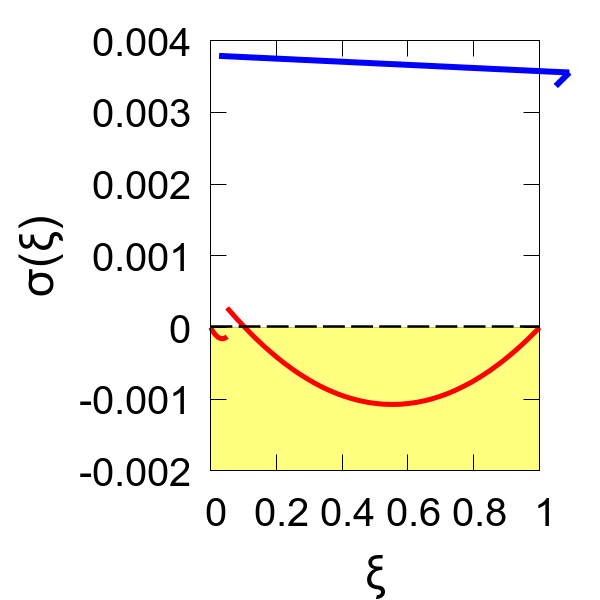
\includegraphics[width=1\textwidth]{plot/tensile_stress/sigma_q_0.45_alpha_0.250pi.png}
		\end{minipage}
		\label{fig:16.f}
	}
	\caption{Tensile stress for different shape parameters ($\mathcal{I}=0$).}
	\label{fig:17}
\end{figure}

Figure \ref{fig:17} presents the six results of the tensile stress for different shape parameters when $\mathcal{I}=0$. When $\xi=0$ or $\xi=1$, $\sigma=0$, which is consistent with the fact that no force acts on the free ends. Each plot shows a jump discontinuity at the hinge point. It can be observed that the tensile stress at this point is non-zero and has opposite signs on either side, indicating a complex mechanical relationship at the hinge. The curves illustrate the tensile stress experienced by the rigid fibre under fluid forces, indicating a tendency for deformation if it were made of elastic material. 

\subsubsection{Non-rotating to rotating solutions: A SNIPER bifurcation}
\begin{figure}[!h]
	\begin{center}
		% specify width as 80% of the width of the text on the page
		% we can also specify a width in centimetres, e.g. [width=8cm]
		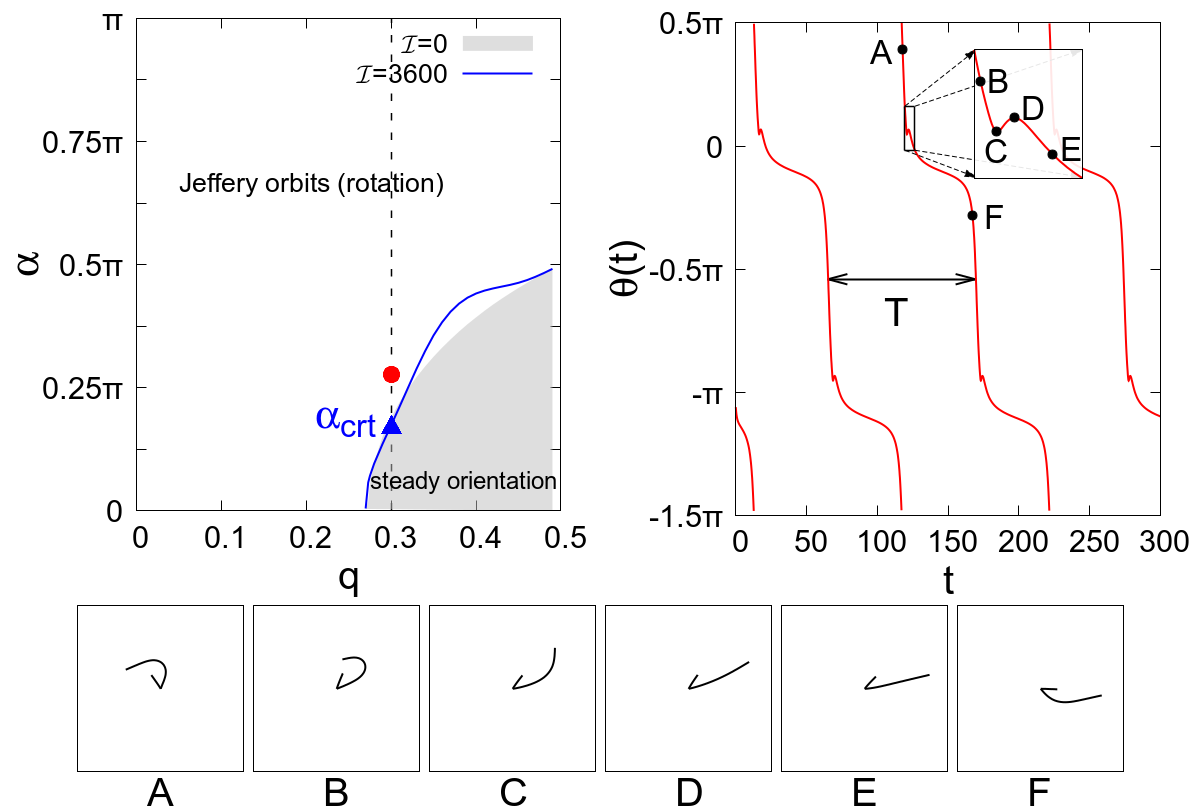
\includegraphics[width=1\textwidth]{plot/rotating_and_non_rotating/rotating.png}
		\caption{Top left: Undeformed configuration of the elastic fibre corresponding to the red point ($q=0.3, \alpha=0.278\pi>\alpha_{crt}$) located in the white region, where the motion follows Jeffery orbits. The blue line marks the boundary of the new steady orientation region for $\mathcal{I}$. Top right: Time evolution of the instantaneous orientation $\theta(t)$ with period $T$. Bottom: Shape of the elastic fibre (actual shape, no stretching) undergoing large flow-induced deformations in shear flow.}
		\label{fig:24}
	\end{center}
	%	\setlength{\abovecaptionskip}{-0.5 cm}
\end{figure}

\begin{figure}[!h]
	\begin{center}
		% specify width as 80% of the width of the text on the page
		% we can also specify a width in centimetres, e.g. [width=8cm]
		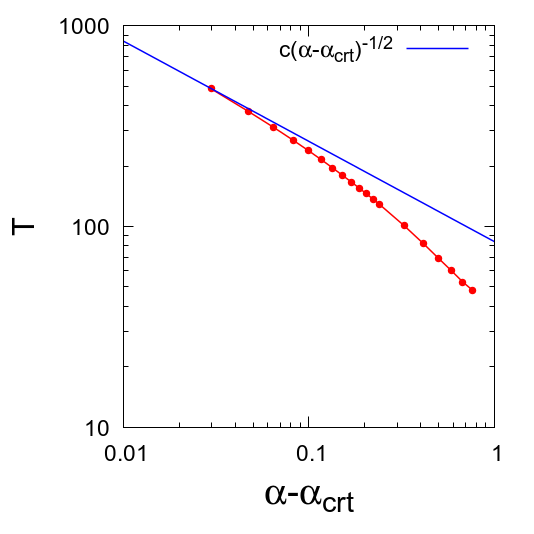
\includegraphics[width=0.6\textwidth]{plot/T_alpha_plots/I_0.0003000_q_0.300_initial_-4.80_element_20_T_alpha_plot_new.png}
		\caption{The numerical results for $q=0.3, \alpha>\alpha_{crt}$ (red line points) asymptotically approach the theoretical prediction of the SNIPER bifurcation.}
		\label{fig:25}
	\end{center}
	%	\setlength{\abovecaptionskip}{-0.5 cm}
\end{figure}

%% End of file `jfm.bib'.


\end{document}
